\documentclass[11pt]{article}
\usepackage[spanish]{babel}
\usepackage[utf8]{inputenc}
\usepackage[nottoc]{tocbibind}

\usepackage{booktabs}  
\usepackage{graphicx} 
\usepackage{listings}
\usepackage{amsmath,amsthm,amssymb}
\usepackage{mathtools}
\usepackage{float}

\usepackage
[
  a4paper,% other options: a3paper, a5paper, etc
  left=1.7cm,
  right=2cm,
  top=3cm,
  bottom=4cm,
]
{geometry}

\lstset{%
backgroundcolor=\color{cyan!10},
basicstyle=\ttfamily,
numbers=left,numberstyle=\scriptsize
}

\setlength{\parskip}{\baselineskip}%
\setlength{\parindent}{0pt}%

%\usepackage[wby]{callouts}
\usepackage{hyperref}
\usepackage{url}

% pseudocode
\usepackage{algpseudocode}
\usepackage{algorithm}
\usepackage{algorithmicx}

\usepackage{graphicx}
\usepackage{caption}
\usepackage{subcaption}


\title{Whale Optimziation Algorithm aplicado al problema de clustering}
\author{Yábir García Benchakhtir}
\begin{document}

\maketitle

\begin{figure}[h]

\includegraphics[scale=0.3]{UGR}
\centering
\end{figure}

\newpage

\renewcommand*\contentsname{Índice}
\tableofcontents

\newpage

\section{Introducción al problema}


Consideramos el problema del agrupamiento con restricciones. En este
problema contamos con un conjunto no vacio $P \subset \mathbb{R}^n$ de
puntos y nos planteamos cómo podríamos agruparlos de manera que exista
una relación entre los puntos de un mismo grupo. A cada grupo lo
denominaremos \textit{cluster} y notaremos $\mathcal{C}$ al conjunto
de todos los clusters.

Sobre esta base imponemos restricciones en la manera en la que se
realizan las agrupaciones. En primer lugar existe un subconjunto de
pares de puntos $ML$ definido como

\[ ML = \{(a,b) \in P\times P\ | \quad a \in K \iff b\in K \text{ para } K \in \mathcal{C}\}\]

es decir, el conjunto de puntos que han de estar en el mismo
cluster. De manera similar existe otro conjunto $CL$ de pares de
puntos que no pueden pertenecer al mismo conjunto.

\[ CL = \{(a,b) \in P\times P\ | \quad a \in K \iff b\notin K \text{ para } K \in \mathcal{C}\}\]

Notaremos por $R = ML \cup CL$ al conjunto de restricciones del problema.

Nos concentraremos en encontrar soluciones bajo restricciones \textit{débiles} a
este problema donde intentaremos encontrar soluciones que minimicen el conjunto
restricciones incumplidas.

En nuestros algoritmos intentaremos minimizar la distancia que haya
entre los puntos de cada cluster sujeto a que se violen el menor
número de restricciones. Vamos a formalizar pues esta idea,
definimos el centroide de un cluster como el punto promedio de los
puntos del cluster

\[
  \mu_i = \frac{1}{|c_i|}\sum_{x\in c_i}x \quad \text{ con } c_i \in \mathcal{C} \text{ para todo } i \in \{1,...k\}
\]

Definimos la distancia \textit{intra-cluster} como la media de las
distancias de cada punto del cluster al centroide. En este caso
consideramos la distancia euclidea.

\[
  \bar c_i = \frac{1}{|c_i|}\sum_{x\in c_i}||x-\mu_i||_2 \quad \text{ con } c_i \in \mathcal{C} \text{ para todo } i \in \{1,...k\}
\]

La desviación general del problema será por tanto

\[
  \bar C = \frac{1}{k}\sum_{c_i\in \mathcal{C}}\bar c_i
\]

Nuestro objetivo cuanto busquemos una solución con restricciones
débiles será minimizar la desviación general sujeto a que "no
incumplamos demasiadas restricciones". Para obtener un valor que le de
mayor o menor relevancia a la cantidad de restricciones que
incumplamos usaremos la siguiente proporción

\[
  \lambda = \frac{\lceil d \rceil}{|R|}
\]

donde $d$ es la mayor distancia entre puntos del conjunto de puntos
$P$.  Así nuestro objetivo,cuando busquemos una solución con
restricciones débiles, será minimizar

\[
  f = \bar C + \lambda * \text{infeasibility}
\]

donde \textit{infeasibility} es la cantidad de restricciones incumplidas.

\section{Whale Optimziation Algorithm}

La metaheurística elegida para resolver el problema ha sido Whale Optimziation
Algorithm (WOA) propuesta por Seyedali Mirjalili y Andrew Lewis en 2016 \cite{woa}. Esta
metaheurística basa su comportamiento en las técnicas depredadoras de la ballena
jorobada y su comportamiento social. 

Utilizando el especial comportamiento que tiene este animal cuando colabora con 
otros de su misma especia se pretende conseguir una metaheurística que proporcione
buenos resultados en problemas de optimización de funciones reales intentando 
preservar un equilibrio entre exploración y explotación.

Más concretamente la técnica de caza consiste en crear una espiral entorno a la 
presa y levantar un \textit{muro} de burbujas de aire, haciendo que esta se desoriente
para posteriormente acercarse y atacar. 

\subsection{Descripción de la metaheurística}

Para modelar el problema los autores de la metaheurística proponen un modelado 
matemático del comportamiento de la ballena jorobada que se pueda adaptar adaptar 
a la optimización de una función real.

Los agentes $X$ que participan en nuestro algoritmo (y que representan a las
ballenas) se van a representar como $N$ vectores de dimensión $d$ donde cada
componente del vector del agente representa el centroide de un cluster

\[
    X_i(t) = <X_{i1}(t), X_{i2}(t), \dots, X_{id}(t)>
\]

Como deja entrever esta notación, el estado de la ballena depende de una variable 
temporal $t$ que representa el instante de tiempo en el que nos encontramos y 
que está limitado por una constante $T$ que fijamos nosotros. En cada instante 
$t$ la mejor solución vendrá representada por $X^*$.

Procedemos en primer lugar a definir el operador distancia entre dos ballenas

\begin{align*}
    ||\cdot||\colon & \mathbb{R}^n\times\mathbb{R}^n \to \mathbb{R}^n\\
    & (<x_1, x_2, \dots, x_n>, <y_1, y_2, \dots, y_n>) \xmapsto{}<|x_1 - y_1|, |x_2-y_2|, \dots, |x_n-y_n|>
\end{align*}

que es la distancia coordenada a coordenada.

El movimiento de caza se representa por la modificación del vector agente
mediante la expresión

\begin{align}
    X_i(t+1) = X^*(t) - A\cdot D_i^1  \label{eq:1}
\end{align}

donde $\cdot$ representa el producto componente a componente de $\mathbb{R}^n$, $D$ viene dado por
la expresión

\[
    D^1_i = ||CX^*(t)-X_i(t)||    
\]

y $A \text{ y } C$ se obtienen como 

\begin{align*}
    A &= 2a\cdot r - a \\
    C &= 2r
\end{align*}

con $r \in [0,1]^d$ un vector aleatorio y $a\in [0,2]^d$ constante que se hace
decrecer de manera lineal a lo largo de los distintos pasos del algoritmo
mediante la ecuación

\[
  a(t) = 2-2\frac{t}{\text{max\_evaluaciones}}  
\]

La técnica de \textit{caza} se basa en combinar este movimiento que nos
proporciona un componente de exploración junto a la creación de una espiral 
mediante la actualización del agente de acuerdo a la expresión 

\begin{align}
\begin{cases}
    X_i(t+1) &= e^{bl}cos(2\pi l)D_2 + X^* \\
    D^2_i &= ||X^*(t)-X_i(t)||\\
\end{cases}\label{eq:2}
\end{align}

siendo $b \in \mathbb{R}$ constante y $l \in [-1,1]$ aleatorio de manera que
nos definen un radio para la espiral en cada instante.

El movimiento de caza natural mezcla tanto los desplazamientos en linea recta
como el comportamiento en espiral por lo que se introduce un factor aleatorio
$p \in [0,1]$ que decide que tipo de movimiento se va a realizar

\[
    X_i(t+1) =  
\begin{cases}
    X^*(t) - A\cdot D^1_i & p < \frac{1}{2}\\
    e^{bl}cos(2\pi l)D^2_i + X^*  & p\geq \frac{1}{2}\\  
\end{cases}
\]

\subsection{Adaptación de la metaheurística al problema}

Durante el desarrollo de la asignatura hemos trabajado con una representación
de la solución que se centraba en la asignación de cada punto a un cluster
y se re-calculaba en cada caso los centros de cada cluster. El espacio de búsqueda 
era 

\[
    \{<x_1, x_2, \dots x_n >: x_i \in [0, k] \cap \mathbb{N}, k > 0\}
\]

donde $n$ representa el número de puntos que intervienen en el problema y k el número 
de clusters que consideramos.

Para adaptar la metaheurística he decidido variar mi enfoque del problema y, en
lugar de modificar las asignaciones que hago de los puntos, pensar que cada
agente representa las coordenadas de los centroiedes del problema.

Así cada agente (ballena) queda definido como 

\[
    X_i = <<c_{01},c_{02}, \dots c_{0d}>, \overset{(k)}{\dots}, <c_{k1},c_{k2},\dots c_{kd}>>    
\]

una lista de $k$ vectores con dimensión $d$, la dimensión de los puntos del
problema. No obstante esto no es suficiente ya que nuestro objetivo final es 
proporcionar una asignación de los puntos a cada cluster. 

El algoritmo WOA se encargará de minimizar la componente real y continua de la
métrica que estamos evaluando (que además tiene más peso en la misma), la
distancia de los centroides respecto a los puntos de cada cluster. La segunda
componente de la métrica es el factor de \textit{infeasibility} que
minimizaremos asignando a cada punto el cluster que menos incremento en
infeasibility produzca y, en caso de empate, el cluster más cercano.

El comportamiento del algoritmo, como se muestra a continuación, es sencillo 

\begin{algorithm}[H]
  \caption{Whale optimization Algorithm}
  \label{alg-lsearch}
  \begin{algorithmic}[1]
    \Procedure{WOA}{max\_evaluaciones}
    \State whales: Inicializar un conjunto de ballenas con k centroides aleatorios
    \State Evaluamos las diferentes ballenas usando nuestra métrica 
    \State Selecccionamos $X^*$ la mejor ballena
    \State Guardamos la mejor solución encontrada al problema
    \State evaluaciones $\leftarrow$ 0
    \While {evaluaciones $<$ max\_evaluaciones }
    \State actualizamos el parametro $a$
    \For{agente en la lista de ballenas}
    \State Determianr $p$ y calcular  $A$ y $C$.
    \If{$p<0.5$}
    \If {$|A| < 1$}
    \State Movemos la ballena usando el movimeinto rectilineo \eqref{eq:1}
    \ElsIf {$|A|>1$} 
    \State Movimiento rectilineo usando una ballena eleatoria \eqref{eq:1}
    \EndIf
    \Else
    \State Movimiento en espiral utilizando \eqref{eq:2}
    \EndIf
    \EndFor 
    \State Comprobar si alguna solución se ha salido de los limites del problema
    \State Incrementar evaluaciones en el número de evaluaciones correspondiente
    \State Evaluar las soluciones encontradas y actualizar la mejor ballena 
    \If{la mejor ballena es la mejor solución encontrada}
    \State Actualizar la mejor solución encontrada hasta el momento
    \EndIf
    \EndWhile
    \State
    \Return Construir la solución asociada a la mejor ballena encontrada
    \EndProcedure
  \end{algorithmic}
\end{algorithm}

El algoritmo que, a partir de una ballena, nos permite crear una solución en el
formato que hemos descrito es 


\begin{algorithm}[H]
  \caption{Generar una solución a partir de un conjunto de centroides}
  \label{alg-lsearch}
  \begin{algorithmic}[1]
    \Procedure{Generar solución}{datos, restricciones, centroides}
    \State clusters $\leftarrow [[]\dots[]]$  Lista con los puntos asociados a cada cluster
    \For{cada punto $p$ del conjunto de datos}
    \State Calcular el coste de infeasibility que supone asignar el punto a los diferentes clusters 
    \State elegir $K = [k_0,\dots,k_s]$ los clusters que menor incremento de infeasibility suponen
    \If {$K.size() == 1$}
    \State Asignar $p$ al cluster $K[0]$
    \Else
    \State Calcular la distancia del punto $p$ al centro de cada cluster $k_i \in K$
    \State Asignar $p$ al cluster más cercano
    \EndIf
    \EndFor
    \State
    \Return Construir la asignación a partir de la lista de puntos en cada cluster
    \EndProcedure
  \end{algorithmic}
\end{algorithm}

Por último describimos en pseudocódigo las funciones que nos permiten evaluar
las soluciones que obtengamos en los distintos experimentos que se han realizado

\begin{algorithm}[H]
  \caption{Calcular el valor de infeasibility para una solución}
  \label{alg-inf}
  \begin{algorithmic}[1]
    \Procedure{calc\_infeasibility(solucion, restricciones)}{}
    \State inf = 0
    \For {$c_i \in \text{sol}$ }
    \State R = Comprobar las relaciones de $c_i$ con el resto de elementos $c_j$ de su cluster
    \For {relacion en R}
    \If {deberían estar juntos y no lo están o están en el mismo cluster sin deberlo }
    \State inf += 1
    \EndIf
    \EndFor
    \EndFor
    \State return inf
    \EndProcedure
  \end{algorithmic}
  \end{algorithm}
  
para calcular el valor de desviación instracluster
  
  \begin{algorithm}[H]
  \caption{Calcular la desviación intracluster}
  \label{alg-intra}
  \begin{algorithmic}[1]
    \Procedure{calc\_c(solucion, puntos, k)}{}
    \State centros = [centros para cada cluster 0...k ]
    \State num = [número de elementos de cada cluster 0...k]
    \State inner = [distancia intra cluster 0...k] inicializado a 0
    \For {i,c $\in$ enumerate(solucion)}
    \State inner[c] += norma\_l2(puntos[i]-centros[c])
    \EndFor
    \State inner = inner/num
    \State return sum(inner)/k
    \EndProcedure
  \end{algorithmic}
  \end{algorithm}
  
  
  también nos hará falta un método para calcular lo que en la
  descripción del problema hemos llamado $\lambda$.
  
  \begin{algorithm}[H]
  \caption{Calcular el valor de $\lambda$ para el problema}
  \label{alg-lambda}
  \begin{algorithmic}[1]
    \Procedure{calc\_lambda(data: conjunto de puntos, rest: matriz de restricciones)}{}
    \State max\_dist $\leftarrow$ 0 
    \For {u $\in$ data}
    \For {v $\in$ data}
    \State d $\leftarrow$ norm 2 of u - v
    \If {d $>$ max\_dist}
    \State max\_dist = d
    \EndIf
    \EndFor
    \EndFor
    \State n $\leftarrow$ contar el número de restricciones no cero
    \State // Eliminamos la diagonal y los puntos duplicados
    \State n $\leftarrow$ (n-rest.size)/2
    \State \Return max\_dist/k
    \EndProcedure
  \end{algorithmic}
  \end{algorithm}
  
  
  La función \textit{score} que nos permite evaluar una
  solución sería
  
  \begin{algorithm}[H]
  \caption{Calcular el score de una solución}
  \label{score}
  \begin{algorithmic}[1]
    \Procedure{calc\_score(sol: Solution, data: conjunto de puntos, rest: matriz de restricciones)}{}
    \State \Return calc\_c(sol, puntos, k) + calc\_lambda(data, rest) * calc\_infeasibility(sol, rest)
    \EndProcedure
  \end{algorithmic}
  \end{algorithm}

\section{Implementación y desarrollo del experimento}

La implementación del código ha sido realizada en el lenguaje de programación
\textit{Rust} ya que ha sido el el usado durante el desarrollo de las anteriores
prácticas, por lo que se ha podido reutilizar código y las ejecuciones han sido
realizadas bajo las mismas optimizaciones en el lenguaje.

Los experimentos han sido ejecutados en un ordenador con las siguientes
características

\begin{itemize}
  \item CPU: Ryzen 5 2600 3.4GHz
  \item RAM: 24GB
  \item SO: Solus OS
\end{itemize}

Cada experimento consistente en la ejecución del algoritmo bajo 5 semillas
distintas (37,42,440,699,752) de las que se han recopilado datos y se han
agregado tomando medias. También se proporcionan en detalle los resultados para
cada ejecución.

El tamaño de la población como hemos estudiado para este tipo de problemas se
recomienda entre 20 y 50 individuos. En mi caso he optado por fijar este valor a
30 individuos a fin de obtener una primera idea del funcionamiento del
algoritmo. El parámetro $b$ de la espiral lo he fijado a 1 ya que es el valor
que se fija en la versión implementada en MATLAB \cite{matlab}. Tras haber
ejecutado el algoritmo los resultados son los siguientes.

\begin{figure}[H]
  \begin{subfigure}{.5\textwidth}
    \centering
    % include first image
    \begin{table}[H]
      \centering
      \resizebox{\textwidth}{!}{
        \begin{tabular}{l|l|l|l|l|}
\cline{2-5}
& \multicolumn{1}{c|}{Iris} & \multicolumn{1}{c|}{Ecoli} & \multicolumn{1}{c|}{Rand} & \multicolumn{1}{c|}{Tyroid}  \\ \hline 
\multicolumn{1}{|l|}{Semilla 37 } &  0.670304  & 13.046238   &  0.715599   &  14.013687 \\ \hline
\multicolumn{1}{|l|}{Semilla 42 } &  0.671846  & 13.140929   &  0.715599   &  13.500604 \\ \hline
\multicolumn{1}{|l|}{Semilla 440 } &  0.656589  & 13.058654   &  0.715599   &  13.295182 \\ \hline
\multicolumn{1}{|l|}{Semilla 699 } &  0.668911  & 13.050045   &  0.715599   &  13.647765 \\ \hline
\multicolumn{1}{|l|}{Semilla 752 } &  0.666602  & 13.026891   &  0.715599   &  13.790620 \\ \hline
\multicolumn{1}{|l|}{ Media } &  0.666851  & 13.064551   &  0.715599   &  13.649572 \\ \hline
\end{tabular}
      }                
    \end{table} 
    \caption{Distancia intracluster}
  \end{subfigure}
  \begin{subfigure}{.5\textwidth}
    \centering
    % include second image
    \begin{table}[H]
      \centering
      \resizebox{\textwidth}{!}{
        \begin{tabular}{l|l|l|l|l|}
\cline{2-5}
& \multicolumn{1}{c|}{Iris} & \multicolumn{1}{c|}{Ecoli} & \multicolumn{1}{c|}{Rand} & \multicolumn{1}{c|}{Tyroid}  \\ \hline 
\multicolumn{1}{|l|}{Semilla 37 } &  42.000000  & 1273.000000   &  0.000000   &  185.000000 \\ \hline
\multicolumn{1}{|l|}{Semilla 42 } &  32.000000  & 1285.000000   &  0.000000   &  204.000000 \\ \hline
\multicolumn{1}{|l|}{Semilla 440 } &  39.000000  & 1298.000000   &  0.000000   &  203.000000 \\ \hline
\multicolumn{1}{|l|}{Semilla 699 } &  48.000000  & 1288.000000   &  0.000000   &  206.000000 \\ \hline
\multicolumn{1}{|l|}{Semilla 752 } &  40.000000  & 1304.000000   &  0.000000   &  191.000000 \\ \hline
\multicolumn{1}{|l|}{ Media } &  40.200000  & 1289.600000   &  0.000000   &  197.800000 \\ \hline
\end{tabular}
      }                
    \end{table}  
    \caption{Infeasibility}
  \end{subfigure}

  \begin{subfigure}{.5\textwidth}
    \centering
    \begin{table}[H]
      \centering
      \resizebox{\textwidth}{!}{
        \begin{tabular}{l|l|l|l|l|}
\cline{2-5}
& \multicolumn{1}{c|}{Iris} & \multicolumn{1}{c|}{Ecoli} & \multicolumn{1}{c|}{Rand} & \multicolumn{1}{c|}{Tyroid}  \\ \hline 
\multicolumn{1}{|l|}{Semilla 37 } &  0.936712  & 47.200253   &  0.715599   &  20.779371 \\ \hline
\multicolumn{1}{|l|}{Semilla 42 } &  0.874824  & 47.616898   &  0.715599   &  20.961143 \\ \hline
\multicolumn{1}{|l|}{Semilla 440 } &  0.903969  & 47.883408   &  0.715599   &  20.719147 \\ \hline
\multicolumn{1}{|l|}{Semilla 699 } &  0.973378  & 47.606503   &  0.715599   &  21.181446 \\ \hline
\multicolumn{1}{|l|}{Semilla 752 } &  0.920325  & 48.012620   &  0.715599   &  20.775734 \\ \hline
\multicolumn{1}{|l|}{ Media } &  0.921842  & 47.663936   &  0.715599   &  20.883368 \\ \hline
\end{tabular}
      }                
    \end{table} 
    \caption{Función objetivo}
  \end{subfigure}
  \begin{subfigure}{.5\textwidth}
    \centering
    \begin{table}[H]
      \centering
      \resizebox{\textwidth}{!}{
        \begin{tabular}{l|l|l|l|l|}
\cline{2-5}
& \multicolumn{1}{c|}{Iris} & \multicolumn{1}{c|}{Ecoli} & \multicolumn{1}{c|}{Rand} & \multicolumn{1}{c|}{Tyroid}  \\ \hline 
\multicolumn{1}{|l|}{Semilla 37 } &  24.114498  & 249.527510   &  24.124850   &  45.735350 \\ \hline
\multicolumn{1}{|l|}{Semilla 42 } &  24.452518  & 243.258400   &  23.513433   &  44.398865 \\ \hline
\multicolumn{1}{|l|}{Semilla 440 } &  23.470268  & 241.543440   &  23.613468   &  44.316753 \\ \hline
\multicolumn{1}{|l|}{Semilla 699 } &  23.512020  & 241.600170   &  23.420820   &  44.240932 \\ \hline
\multicolumn{1}{|l|}{Semilla 752 } &  23.493227  & 241.310170   &  23.466751   &  44.134445 \\ \hline
\multicolumn{1}{|l|}{ Media } &  23.808506  & 243.447938   &  23.627864   &  44.565269 \\ \hline
\end{tabular}
      }                
    \end{table} 
    \caption{Tiempo de ejecución}
  \end{subfigure}
  \caption{ Resultados para woa con 10\% de restricciones }
  \label{fig:fig}
\end{figure}
\begin{figure}[H]
  \begin{subfigure}{.5\textwidth}
    \centering
    % include first image
    \begin{table}[H]
      \centering
      \resizebox{\textwidth}{!}{
        \begin{tabular}{l|l|l|l|l|}
\cline{2-5}
& \multicolumn{1}{c|}{Iris} & \multicolumn{1}{c|}{Ecoli} & \multicolumn{1}{c|}{Rand} & \multicolumn{1}{c|}{Tyroid}  \\ \hline 
\multicolumn{1}{|l|}{Semilla 37 } &  0.684892  & 12.979752   &  0.715599   &  13.340351 \\ \hline
\multicolumn{1}{|l|}{Semilla 42 } &  0.663448  & 13.042139   &  0.715599   &  13.592555 \\ \hline
\multicolumn{1}{|l|}{Semilla 440 } &  0.662933  & 13.033968   &  0.715599   &  13.620830 \\ \hline
\multicolumn{1}{|l|}{Semilla 699 } &  0.660625  & 13.035360   &  0.715599   &  13.909627 \\ \hline
\multicolumn{1}{|l|}{Semilla 752 } &  0.658393  & 13.160732   &  0.715599   &  13.623517 \\ \hline
\multicolumn{1}{|l|}{ Media } &  0.666058  & 13.050390   &  0.715599   &  13.617376 \\ \hline
\end{tabular}
      }                
    \end{table} 
    \caption{Distancia intracluster}
  \end{subfigure}
  \begin{subfigure}{.5\textwidth}
    \centering
    % include second image
    \begin{table}[H]
      \centering
      \resizebox{\textwidth}{!}{
        \begin{tabular}{l|l|l|l|l|}
\cline{2-5}
& \multicolumn{1}{c|}{Iris} & \multicolumn{1}{c|}{Ecoli} & \multicolumn{1}{c|}{Rand} & \multicolumn{1}{c|}{Tyroid}  \\ \hline 
\multicolumn{1}{|l|}{Semilla 37 } &  77.000000  & 2637.000000   &  0.000000   &  371.000000 \\ \hline
\multicolumn{1}{|l|}{Semilla 42 } &  55.000000  & 2553.000000   &  0.000000   &  294.000000 \\ \hline
\multicolumn{1}{|l|}{Semilla 440 } &  81.000000  & 2663.000000   &  0.000000   &  426.000000 \\ \hline
\multicolumn{1}{|l|}{Semilla 699 } &  76.000000  & 2512.000000   &  0.000000   &  337.000000 \\ \hline
\multicolumn{1}{|l|}{Semilla 752 } &  90.000000  & 2625.000000   &  0.000000   &  348.000000 \\ \hline
\multicolumn{1}{|l|}{ Media } &  75.800000  & 2598.000000   &  0.000000   &  355.200000 \\ \hline
\end{tabular}
      }                
    \end{table}  
    \caption{Infeasibility}
  \end{subfigure}

  \begin{subfigure}{.5\textwidth}
    \centering
    \begin{table}[H]
      \centering
      \resizebox{\textwidth}{!}{
        \begin{tabular}{l|l|l|l|l|}
\cline{2-5}
& \multicolumn{1}{c|}{Iris} & \multicolumn{1}{c|}{Ecoli} & \multicolumn{1}{c|}{Rand} & \multicolumn{1}{c|}{Tyroid}  \\ \hline 
\multicolumn{1}{|l|}{Semilla 37 } &  0.928991  & 48.354507   &  0.715599   &  20.122843 \\ \hline
\multicolumn{1}{|l|}{Semilla 42 } &  0.837804  & 47.290054   &  0.715599   &  18.967363 \\ \hline
\multicolumn{1}{|l|}{Semilla 440 } &  0.919712  & 48.757507   &  0.715599   &  21.408813 \\ \hline
\multicolumn{1}{|l|}{Semilla 699 } &  0.901553  & 46.733270   &  0.715599   &  20.070543 \\ \hline
\multicolumn{1}{|l|}{Semilla 752 } &  0.943702  & 48.374510   &  0.715599   &  19.985538 \\ \hline
\multicolumn{1}{|l|}{ Media } &  0.906353  & 47.901970   &  0.715599   &  20.111020 \\ \hline
\end{tabular}
      }                
    \end{table} 
    \caption{Función objetivo}
  \end{subfigure}
  \begin{subfigure}{.5\textwidth}
    \centering
    \begin{table}[H]
      \centering
      \resizebox{\textwidth}{!}{
        \begin{tabular}{l|l|l|l|l|}
\cline{2-5}
& \multicolumn{1}{c|}{Iris} & \multicolumn{1}{c|}{Ecoli} & \multicolumn{1}{c|}{Rand} & \multicolumn{1}{c|}{Tyroid}  \\ \hline 
\multicolumn{1}{|l|}{Semilla 37 } &  28.139378  & 293.534940   &  28.877132   &  53.587063 \\ \hline
\multicolumn{1}{|l|}{Semilla 42 } &  28.537369  & 284.490780   &  27.549004   &  52.060455 \\ \hline
\multicolumn{1}{|l|}{Semilla 440 } &  27.767319  & 283.893800   &  27.526875   &  52.108093 \\ \hline
\multicolumn{1}{|l|}{Semilla 699 } &  27.650816  & 283.500640   &  27.543203   &  52.094227 \\ \hline
\multicolumn{1}{|l|}{Semilla 752 } &  27.724705  & 282.832120   &  27.512619   &  51.931313 \\ \hline
\multicolumn{1}{|l|}{ Media } &  27.963917  & 285.650456   &  27.801767   &  52.356230 \\ \hline
\end{tabular}
      }                
    \end{table} 
    \caption{Tiempo de ejecución}
  \end{subfigure}
  \caption{ Resultados para woa con 20\% de restricciones }
  \label{fig:fig}
\end{figure}

\section{Análisis de los resultados}

En primer lugar vamos a proceder a comparar los resultados obtenidos con los
resultados usando otros algoritmos desarrollados durante el curso. La lista de
algoritmos con la que vamos a comparar es 

\begin{itemize}
  \item greedy: Versión greedy
  \item ls: Busqueda local 
  \item age-fs: Algoritmo genético estacionario con cruce de segmento fijo 
  \item age-u: Algoritmo genético estacionario con cruce uniforme
  \item agg-fs: Algoritmo genético generacional con cruce de segmento fijo 
  \item agg-u: Algoritmo genético generacional con cruce uniforme
  \item am-*: Algoritmo memético en diferentes variantes de los paráemtros 
  \item es: Enfriamiento simulado
  \item bmb: Busqueda multiarranque básica
  \item ils: Búsqueda local iterativa
  \item ils-es: Búsqueda local iterativa con enfriamiento simulado
\end{itemize}

\begin{table}[H]
  \centering
  \resizebox{\textwidth}{!}{
  \begin{tabular}{|l|l|l|l|l|l|l|l|l|l|l|l|l|}
    \hline
    & \multicolumn{3}{c}{Iris} & \multicolumn{3}{|c}{Ecoli} & \multicolumn{3}{|c}{Rand}& \multicolumn{3}{|c|}{Newthyroid} \\ \hline
    & tasa C  & inf & score  & tasa C & inf & score & tasa C & inf  & score & tasa C & inf & score\\ \hline 
    greedy & 1.800 & 355.8 & 4.057 & 44.613 & 1500.4 & 84.868  & 2.227 & 299.4 & 4.383 &13.160  &958.2 & 48.203\\ \hline
    ls & 0.669 & 0.000  & 0.669 & 21.604 & 92.200 & 24.078 & 0.716  &0.000  &0.716  & 13.246  &24.4 & 14.138\\ \hline
    age-fs & 0.669 & 0.000 & 0.669  & 21.291 &94.000  & 23.813 & 0.716  & 0.000 &0.716  &12.043  & 63.600 & 14.369\\ \hline
    age-u & 0.669 & 0.000 & 0.669 & 21.622 & 97.800 & 24.246 & 0.716 & 0.000 & 0.716 &12.038 & 67.000  &14.488\\ \hline
    agg-fs & 0.671	 & 4.000 & 0.696 & 22.855  & 146.60  & 26.788 & 0.723  & 4.200 & 0.753 &13.835  & 6.000 &14.054 \\ \hline
    agg-u & 0.669 & 0.000  & 0.669 & 22.617  & 141.80 & 26.422 & 0.716 & 0.000 & 0.716 & 12.645 & 51.800 &14.539\\ \hline
    am-01 & 0.669 & 0.000 & 0.669  &23.726  & 98.200  & 26.360 & 0.716 &0.000  & 0.716	 & 12.037 & 68.200 &14.531\\ \hline
    am-all & 0.671 & 1.800 & 0.682 & 22.759 & 97.600 & 25.377 &0.719  & 1.000 & 0.727 &12.036  & 61.200& 14.275\\ \hline
    am-top-01 & 0.669  & 0.000 & 0.669 & 21.929 & 125.00 &25.283  & 0.716	 &0.000  &0.716  & 12.070&65.800 &14.476 \\ \hline
    es & 0.669 & 0.000  & 0.669 & 21.679 & 83.800 & 23.927 & 0.716  & 0.000 & 0.716 & 12.628  & 47.400 & 14.362  \\ \hline
    bmb & 0.669 & 0.000  & 0.669 & 21.997 & 156.000 & 26.183 & 0.716  & 0.000 & 0.716 & 13.835	 & 6.000 & 14.054 \\ \hline
    ils & 0.669 & 0.000  & 0.669 & 21.781 & 75.800 & 23.815	 & 0.716 & 0.000 & 0.716 & 13.835  & 6.000 & 14.054  \\ \hline
    ils-es & 0.669 & 0.000  & 0.669 &  28.198 & 332.800	 & 37.127 & 0.716 & 0.000  & 0.716 &  13.835 & 6.000 & 14.054  \\ \hline
    woa & 0.667 	 & 40.200  & 0.922 &  13.065 & 1289.600 & 47.664 & 0.716 & 0.000  & 0.716 &  13.650 & 197.800  &  	20.883 \\ \hline


  \end{tabular}}
  \caption{Resultados medios obtenidos para el problema del PAR con restricciones del 10\%}
\end{table}

\begin{table}[H]
  \centering
  \resizebox{\textwidth}{!}{
  \begin{tabular}{|l|l|l|l|l|l|l|l|l|l|l|l|l|}
    \hline
    & \multicolumn{3}{c}{Iris} & \multicolumn{3}{|c}{Ecoli} & \multicolumn{3}{|c}{Rand}& \multicolumn{3}{|c|}{Newthyroid} \\ \hline
    & tasa C  & inf & score  & tasa C & inf & score & tasa C & inf  & score & tasa C & inf & score\\ \hline 
    greedy &1.686  &690.4  &3.874  &44.953  &3166.6  & 87.433 & 2.332 & 667.8  & 4.735 & 13.200 &2056.4  & 50.795 \\ \hline
    ls & 0.669 & 0.000 & 0.669 & 21.828 & 167.6 &24.076  &  0.716  & 0.000 & 0.716  &12.215  &152.0  & 14.994 \\ \hline
    age-fs &0.669  & 0.000 &0.669  &22.000	  &158.200  & 24.122 &0.716  & 0.000  & 0.716 & 12.896  &95.80  & 14.647  \\ \hline
    age-u& 0.669 & 0.000 & 0.669 & 21.346 & 194.400 & 23.954 & 0.716 & 0.000  & 0.716 & 12.911 &97.00  & 14.684 \\ \hline
    agg-fs& 0.675 & 8.600 & 0.702 & 22.330 &192.800  & 24.916 & 0.737 & 13.00  & 0.783  &12.908	  & 98.0 & 14.699  \\ \hline
    agg-u&0.669  & 0.000 &0.669  &22.607  &209.400  &25.416  &0.716  & 0.000 & 0.716 &12.744  &151.20  & 15.508  \\ \hline
    am-01& 0.669 & 0.000 & 0.669 & 22.186 & 211.400 &25.021  & 0.716 & 0.000  & 0.716 &13.026  &152.00  & 15.805 \\ \hline
    am-all& 0.676 & 5.000 &0.692  &21.965  & 160.400 & 24.116 & 0.720 & 4.800 & 0.738 &12.893  & 91.80 & 14.572 \\ \hline
    am-top-01&0.669  & 0.000 &0.669  &22.986  & 201.200  &25.685  & 0.716 & 0.000 & 0.716 &12.453  &156.8  & 15.320 \\ \hline
    es & 0.669 & 0.000  & 0.669 & 21.849 & 	179.000 & 24.250 &  0.716	 & 0.000 & 0.716 & 12.206 & 159.000 & 15.112 \\ \hline
    bmb & 0.669 & 0.000  & 0.669 & 22.428	  & 224.400	 & 25.439 &  0.716 & 0.000 & 0.716 & 14.287 & 0.000 & 14.287 \\ \hline
    ils & 0.669 & 0.000  & 0.669 &  21.826 & 182.400 & 24.273	 & 0.716 & 0.000 & 0.716 & 14.287 & 0.000 & 14.287 \\ \hline
    ils-es & 0.669 & 0.000  & 0.669 & 28.232  & 	646.400 & 36.903 &  0.716 & 0.000 & 0.716 & 14.287 & 0.000 & 14.287 \\ \hline
    woa & 0.666 & 75.800  & 0.906 &  13.050 & 2598.000 & 47.902 & 0.716 & 0.000  & 0.716 &  13.617 & 355.200 & 20.111  \\ \hline

  \end{tabular}}
  \caption{Resultados medios obtenidos para el problema del PAR con restricciones del 20\%}
\end{table}

Viendo estos resultados comprobamos como el algoritmo efectivamente hace un buen
trabajo reduciendo la distancia intracluster que era la parte que optimizaba el
algoritmo pero sin embargo la solución empeora de manera considerable ya que la
asignación que se hace de los puntos provoca que se incumplan muchas restricciones.

También como se muestra en este histórico de datos generado para el problema de
ecoli con un 10\% de restricciones se encuentran de manera sucesiva mejores
soluciones en etapas tempranas de la ejecución pero después la calidad de las
soluciones no mejora de manera considerable aún estando lejos del óptimo conocido. 

\begin{figure}[H]
  \centering
  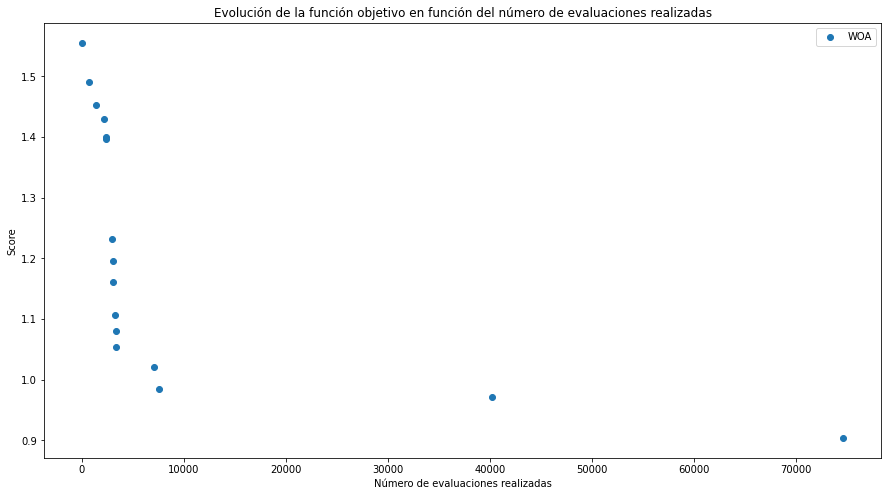
\includegraphics[width=0.8\textwidth]{images/evolution}
  \caption{Evolución de la función objetivo en función del número de evaluaciones}
\end{figure}
  

Este comportamiento se explica ya que los agentes de la búsqueda comienzan a
desplazarse en entornos cercanos a ellos y no exploran realmente el espacio de
búsqueda de manera eficiente. 

Una primera solución que planteo al problema es la hibridación con una búsqueda
local. El motivo es que los centroides creados ya optimizan bien la distancia de
los centros a los puntos pero no el valor de infeasibility. Con una búsqueda
local podemos modificar las soluciones de manera que se mejore el factor de
infeasibility y se mantengan buenos resultados en lo que a las distancias se refiere.

\section{Modificación I: Búsqueda local}

\subsection{Descripción de los cambios}

Como se ha comentado anteriormente he decidido hibridar el algoritmo con una
búsqueda local para mejorar el factor de infeasibility en las soluciones. He
decidido reutilizar la búsqueda local que hemos utilizado en otras prácticas y
que queda descrita en el siguiente código.

\begin{algorithm}[H]
  \caption{Aplicación de la búsqueda local al problema de clustering con restricciones}
  \label{alg-lsearch}
  \begin{algorithmic}[1]
    \Procedure{LS}{}
    \State clusters = \{1,2,\dots k\}
    \State solucion = $<s_1,s_2, \dots,s_n>$
    \State saltos = 0
    \State l = computeLambda(points, restrictions)
    \State cambiosPosibles = $<(id,nuevo\_c)>$
    \For{ $i \in \mathbb{Z}^+ : i \leq \text{max\_iters}$ }
    \If {size(cambiosPosibles) = 0}
    \State return solucion, infeasibility, tasac, puntuacion
    \EndIf
    \State j,c = Pop(cambiosPosibles)
    \State newSol = solucion where $solucion[j]\rightarrow c$
    \State Comprobar que la solución no deja ningun cluster vacio
    \If {$score(newSol) < \text{score actual}$}
    \State solucion = newSol
    \State actualizar score actual
    \State crear nueva permutacion de cambios
    \State saltos += 1
    \EndIf
    \EndFor
    \State Calcular centroides a partir de la solución 
    \State 
    \Return centroides, solución, puntuación
    \EndProcedure
  \end{algorithmic}
  \end{algorithm}

En nuestro algoritmo introduciremos al final de cada iteración del mismo una
pequeña búsqueda local al mejor de los agentes. La idea con esto es que la
ballena guía mejore y arrastre al resto con ellas. La actualización del
pseudocódigo sería la siguiente


\begin{algorithm}[H]
  \caption{Whale optimization Algorithm + LS}
  \label{alg-lsearch}
  \begin{algorithmic}[1]
    \Procedure{WOA-LS}{max\_evaluaciones}
    \State whales: Inicializar un conjunto de ballenas con k centroides aleatorios
    \State Evaluamos las diferentes ballenas usando nuestra métrica 
    \State Seleccionamos $X^*$ la mejor ballena
    \State Guardamos la mejor solución encontrada al problema
    \State evaluaciones $\leftarrow$ 0
    \While {evaluaciones $<$ max\_evaluaciones }
    \State actualizamos el parámetro $a$
    \For{agente en la lista de ballenas}
    \State Determinar $p$ y calcular  $A$ y $C$.
    \If{$p<0.5$}
    \If {$|A| < 1$}
    \State Movemos la ballena usando el movimiento rectilíneo \eqref{eq:1}
    \ElsIf {$|A|>1$} 
    \State Movimiento rectilíneo usando una ballena aleatoria \eqref{eq:1}
    \EndIf
    \Else
    \State Movimiento en espiral utilizando \eqref{eq:2}
    \EndIf
    \EndFor 
    \State Comprobar si alguna solución se ha salido de los limites del problema
    \State Incremenetar evaluaciones en el número de evaluaciones correspondiente
    \State Evaluar las soluciones encontradas y actualizar la mejor ballena 
    \State Aplicar busqueda local a la mejor ballena encontrada
    \If{la mejor ballena es la mejor solución encontrada}
    \State Actualizar la mejor solución encontrada hasta el momento
    \EndIf
    \EndWhile
    \State
    \Return Construir la solución asociada a la mejor ballena encontrada
    \EndProcedure
  \end{algorithmic}
\end{algorithm}

\subsection{Experimentación}

Volviendo a ejecutar el conjunto de tests con la nueva implementación obtenemos
los siguientes resultados

\begin{figure}[H]
  \begin{subfigure}{.5\textwidth}
    \centering
    % include first image
    \begin{table}[H]
      \centering
      \resizebox{\textwidth}{!}{
        \begin{tabular}{l|l|l|l|l|}
\cline{2-5}
& \multicolumn{1}{c|}{Iris} & \multicolumn{1}{c|}{Ecoli} & \multicolumn{1}{c|}{Rand} & \multicolumn{1}{c|}{Tyroid}  \\ \hline 
\multicolumn{1}{|l|}{Semilla 37 } &  0.669305  & 18.316225   &  0.715599   &  13.834984 \\ \hline
\multicolumn{1}{|l|}{Semilla 42 } &  0.669305  & 22.455173   &  0.715599   &  13.834984 \\ \hline
\multicolumn{1}{|l|}{Semilla 440 } &  0.669305  & 18.724802   &  0.715599   &  13.834984 \\ \hline
\multicolumn{1}{|l|}{Semilla 699 } &  0.669305  & 19.889406   &  0.715599   &  13.834984 \\ \hline
\multicolumn{1}{|l|}{Semilla 752 } &  0.669305  & 18.931786   &  0.715599   &  13.834984 \\ \hline
\multicolumn{1}{|l|}{ Media } &  0.669305  & 19.663478   &  0.715599   &  13.834984 \\ \hline
\end{tabular}
      }                
    \end{table} 
    \caption{Distancia intracluster}
  \end{subfigure}
  \begin{subfigure}{.5\textwidth}
    \centering
    % include second image
    \begin{table}[H]
      \centering
      \resizebox{\textwidth}{!}{
        \begin{tabular}{l|l|l|l|l|}
\cline{2-5}
& \multicolumn{1}{c|}{Iris} & \multicolumn{1}{c|}{Ecoli} & \multicolumn{1}{c|}{Rand} & \multicolumn{1}{c|}{Tyroid}  \\ \hline 
\multicolumn{1}{|l|}{Semilla 37 } &  0.000000  & 314.000000   &  0.000000   &  6.000000 \\ \hline
\multicolumn{1}{|l|}{Semilla 42 } &  0.000000  & 246.000000   &  0.000000   &  6.000000 \\ \hline
\multicolumn{1}{|l|}{Semilla 440 } &  0.000000  & 412.000000   &  0.000000   &  6.000000 \\ \hline
\multicolumn{1}{|l|}{Semilla 699 } &  0.000000  & 362.000000   &  0.000000   &  6.000000 \\ \hline
\multicolumn{1}{|l|}{Semilla 752 } &  0.000000  & 446.000000   &  0.000000   &  6.000000 \\ \hline
\multicolumn{1}{|l|}{ Media } &  0.000000  & 356.000000   &  0.000000   &  6.000000 \\ \hline
\end{tabular}
      }                
    \end{table}  
    \caption{Infeasibility}
  \end{subfigure}

  \begin{subfigure}{.5\textwidth}
    \centering
    \begin{table}[H]
      \centering
      \resizebox{\textwidth}{!}{
        \begin{tabular}{l|l|l|l|l|}
\cline{2-5}
& \multicolumn{1}{c|}{Iris} & \multicolumn{1}{c|}{Ecoli} & \multicolumn{1}{c|}{Rand} & \multicolumn{1}{c|}{Tyroid}  \\ \hline 
\multicolumn{1}{|l|}{Semilla 37 } &  0.669305  & 26.740704   &  0.715599   &  14.054409 \\ \hline
\multicolumn{1}{|l|}{Semilla 42 } &  0.669305  & 29.055243   &  0.715599   &  14.054409 \\ \hline
\multicolumn{1}{|l|}{Semilla 440 } &  0.669305  & 29.778576   &  0.715599   &  14.054409 \\ \hline
\multicolumn{1}{|l|}{Semilla 699 } &  0.669305  & 29.601702   &  0.715599   &  14.054409 \\ \hline
\multicolumn{1}{|l|}{Semilla 752 } &  0.669305  & 30.897762   &  0.715599   &  14.054409 \\ \hline
\multicolumn{1}{|l|}{ Media } &  0.669305  & 29.214797   &  0.715599   &  14.054409 \\ \hline
\end{tabular}
      }                
    \end{table} 
    \caption{Función objetivo}
  \end{subfigure}
  \begin{subfigure}{.5\textwidth}
    \centering
    \begin{table}[H]
      \centering
      \resizebox{\textwidth}{!}{
        \begin{tabular}{l|l|l|l|l|}
\cline{2-5}
& \multicolumn{1}{c|}{Iris} & \multicolumn{1}{c|}{Ecoli} & \multicolumn{1}{c|}{Rand} & \multicolumn{1}{c|}{Tyroid}  \\ \hline 
\multicolumn{1}{|l|}{Semilla 37 } &  1.130866  & 13.205993   &  0.730077   &  3.700471 \\ \hline
\multicolumn{1}{|l|}{Semilla 42 } &  1.112652  & 13.307362   &  0.775028   &  3.672802 \\ \hline
\multicolumn{1}{|l|}{Semilla 440 } &  1.134597  & 13.307977   &  0.740447   &  3.554318 \\ \hline
\multicolumn{1}{|l|}{Semilla 699 } &  1.109715  & 13.379734   &  0.736017   &  3.714991 \\ \hline
\multicolumn{1}{|l|}{Semilla 752 } &  1.071018  & 13.714466   &  0.808268   &  3.690543 \\ \hline
\multicolumn{1}{|l|}{ Media } &  1.111769  & 13.383106   &  0.757967   &  3.666625 \\ \hline
\end{tabular}
      }                
    \end{table} 
    \caption{Tiempo de ejecución}
  \end{subfigure}
  \caption{ Resultados para woa-ls con 10\% de restricciones }
  \label{fig:fig}
\end{figure}
\begin{figure}[H]
  \begin{subfigure}{.5\textwidth}
    \centering
    % include first image
    \begin{table}[H]
      \centering
      \resizebox{\textwidth}{!}{
        \begin{tabular}{l|l|l|l|l|}
\cline{2-5}
& \multicolumn{1}{c|}{Iris} & \multicolumn{1}{c|}{Ecoli} & \multicolumn{1}{c|}{Rand} & \multicolumn{1}{c|}{Tyroid}  \\ \hline 
\multicolumn{1}{|l|}{Semilla 37 } &  0.669305  & 19.030159   &  0.715599   &  14.287071 \\ \hline
\multicolumn{1}{|l|}{Semilla 42 } &  0.669305  & 21.108610   &  0.715599   &  14.287071 \\ \hline
\multicolumn{1}{|l|}{Semilla 440 } &  0.669305  & 14.186336   &  0.715599   &  14.287071 \\ \hline
\multicolumn{1}{|l|}{Semilla 699 } &  0.669305  & 18.974272   &  0.715599   &  14.287071 \\ \hline
\multicolumn{1}{|l|}{Semilla 752 } &  0.669305  & 25.243597   &  0.715599   &  14.287071 \\ \hline
\multicolumn{1}{|l|}{ Media } &  0.669305  & 19.708595   &  0.715599   &  14.287071 \\ \hline
\end{tabular}
      }                
    \end{table} 
    \caption{Distancia intracluster}
  \end{subfigure}
  \begin{subfigure}{.5\textwidth}
    \centering
    % include second image
    \begin{table}[H]
      \centering
      \resizebox{\textwidth}{!}{
        \begin{tabular}{l|l|l|l|l|}
\cline{2-5}
& \multicolumn{1}{c|}{Iris} & \multicolumn{1}{c|}{Ecoli} & \multicolumn{1}{c|}{Rand} & \multicolumn{1}{c|}{Tyroid}  \\ \hline 
\multicolumn{1}{|l|}{Semilla 37 } &  0.000000  & 961.000000   &  0.000000   &  0.000000 \\ \hline
\multicolumn{1}{|l|}{Semilla 42 } &  0.000000  & 635.000000   &  0.000000   &  0.000000 \\ \hline
\multicolumn{1}{|l|}{Semilla 440 } &  0.000000  & 1315.000000   &  0.000000   &  0.000000 \\ \hline
\multicolumn{1}{|l|}{Semilla 699 } &  0.000000  & 872.000000   &  0.000000   &  0.000000 \\ \hline
\multicolumn{1}{|l|}{Semilla 752 } &  0.000000  & 430.000000   &  0.000000   &  0.000000 \\ \hline
\multicolumn{1}{|l|}{ Media } &  0.000000  & 842.600000   &  0.000000   &  0.000000 \\ \hline
\end{tabular}
      }                
    \end{table}  
    \caption{Infeasibility}
  \end{subfigure}

  \begin{subfigure}{.5\textwidth}
    \centering
    \begin{table}[H]
      \centering
      \resizebox{\textwidth}{!}{
        \begin{tabular}{l|l|l|l|l|}
\cline{2-5}
& \multicolumn{1}{c|}{Iris} & \multicolumn{1}{c|}{Ecoli} & \multicolumn{1}{c|}{Rand} & \multicolumn{1}{c|}{Tyroid}  \\ \hline 
\multicolumn{1}{|l|}{Semilla 37 } &  0.669305  & 31.921757   &  0.715599   &  14.287070 \\ \hline
\multicolumn{1}{|l|}{Semilla 42 } &  0.669305  & 29.626990   &  0.715599   &  14.287070 \\ \hline
\multicolumn{1}{|l|}{Semilla 440 } &  0.669305  & 31.826760   &  0.715599   &  14.287070 \\ \hline
\multicolumn{1}{|l|}{Semilla 699 } &  0.669305  & 30.671955   &  0.715599   &  14.287070 \\ \hline
\multicolumn{1}{|l|}{Semilla 752 } &  0.669305  & 31.011951   &  0.715599   &  14.287070 \\ \hline
\multicolumn{1}{|l|}{ Media } &  0.669305  & 31.011883   &  0.715599   &  14.287070 \\ \hline
\end{tabular}
      }                
    \end{table} 
    \caption{Función objetivo}
  \end{subfigure}
  \begin{subfigure}{.5\textwidth}
    \centering
    \begin{table}[H]
      \centering
      \resizebox{\textwidth}{!}{
        \begin{tabular}{l|l|l|l|l|}
\cline{2-5}
& \multicolumn{1}{c|}{Iris} & \multicolumn{1}{c|}{Ecoli} & \multicolumn{1}{c|}{Rand} & \multicolumn{1}{c|}{Tyroid}  \\ \hline 
\multicolumn{1}{|l|}{Semilla 37 } &  1.354837  & 17.762445   &  0.877928   &  5.598342 \\ \hline
\multicolumn{1}{|l|}{Semilla 42 } &  1.373990  & 17.955004   &  0.887015   &  5.543451 \\ \hline
\multicolumn{1}{|l|}{Semilla 440 } &  1.488169  & 17.845692   &  0.901323   &  5.174853 \\ \hline
\multicolumn{1}{|l|}{Semilla 699 } &  1.408770  & 17.817894   &  0.935871   &  5.476333 \\ \hline
\multicolumn{1}{|l|}{Semilla 752 } &  1.363122  & 18.403723   &  0.971957   &  5.329753 \\ \hline
\multicolumn{1}{|l|}{ Media } &  1.397778  & 17.956952   &  0.914819   &  5.424546 \\ \hline
\end{tabular}
      }                
    \end{table} 
    \caption{Tiempo de ejecución}
  \end{subfigure}
  \caption{ Resultados para woa-ls con 20\% de restricciones }
  \label{fig:fig}
\end{figure}

\subsection{Análisis}

\begin{table}[H]
  \centering
  \resizebox{\textwidth}{!}{
  \begin{tabular}{|l|l|l|l|l|l|l|l|l|l|l|l|l|}
    \hline
    & \multicolumn{3}{c}{Iris} & \multicolumn{3}{|c}{Ecoli} & \multicolumn{3}{|c}{Rand}& \multicolumn{3}{|c|}{Newthyroid} \\ \hline
    & tasa C  & inf & score  & tasa C & inf & score & tasa C & inf  & score & tasa C & inf & score\\ \hline 
    greedy & 1.800 & 355.8 & 4.057 & 44.613 & 1500.4 & 84.868  & 2.227 & 299.4 & 4.383 &13.160  &958.2 & 48.203\\ \hline
    ls & 0.669 & 0.000  & 0.669 & 21.604 & 92.200 & 24.078 & 0.716  &0.000  &0.716  & 13.246  &24.4 & 14.138\\ \hline
    age-fs & 0.669 & 0.000 & 0.669  & 21.291 &94.000  & 23.813 & 0.716  & 0.000 &0.716  &12.043  & 63.600 & 14.369\\ \hline
    age-u & 0.669 & 0.000 & 0.669 & 21.622 & 97.800 & 24.246 & 0.716 & 0.000 & 0.716 &12.038 & 67.000  &14.488\\ \hline
    agg-fs & 0.671	 & 4.000 & 0.696 & 22.855  & 146.60  & 26.788 & 0.723  & 4.200 & 0.753 &13.835  & 6.000 &14.054 \\ \hline
    agg-u & 0.669 & 0.000  & 0.669 & 22.617  & 141.80 & 26.422 & 0.716 & 0.000 & 0.716 & 12.645 & 51.800 &14.539\\ \hline
    am-01 & 0.669 & 0.000 & 0.669  &23.726  & 98.200  & 26.360 & 0.716 &0.000  & 0.716	 & 12.037 & 68.200 &14.531\\ \hline
    am-all & 0.671 & 1.800 & 0.682 & 22.759 & 97.600 & 25.377 &0.719  & 1.000 & 0.727 &12.036  & 61.200& 14.275\\ \hline
    am-top-01 & 0.669  & 0.000 & 0.669 & 21.929 & 125.00 &25.283  & 0.716	 &0.000  &0.716  & 12.070&65.800 &14.476 \\ \hline
    es & 0.669 & 0.000  & 0.669 & 21.679 & 83.800 & 23.927 & 0.716  & 0.000 & 0.716 & 12.628  & 47.400 & 14.362  \\ \hline
    bmb & 0.669 & 0.000  & 0.669 & 21.997 & 156.000 & 26.183 & 0.716  & 0.000 & 0.716 & 13.835	 & 6.000 & 14.054 \\ \hline
    ils & 0.669 & 0.000  & 0.669 & 21.781 & 75.800 & 23.815	 & 0.716 & 0.000 & 0.716 & 13.835  & 6.000 & 14.054  \\ \hline
    ils-es & 0.669 & 0.000  & 0.669 &  28.198 & 332.800	 & 37.127 & 0.716 & 0.000  & 0.716 &  13.835 & 6.000 & 14.054  \\ \hline
    woa & 0.667 	 & 40.200  & 0.922 &  13.065 & 1289.600 & 47.664 & 0.716 & 0.000  & 0.716 &  13.650 & 197.800  &  	20.883 \\ \hline
    woa-ls & 0.669 & 0.000  & 0.669 &  19.663 & 356.000  & 29.215 & 0.716 & 0.000  & 0.716 &   	 	13.835 & 6.000 &  	14.054  \\ \hline


  \end{tabular}}
  \caption{Resultados medios obtenidos para el problema del PAR con restricciones del 10\%}
\end{table}

\begin{table}[H]
  \centering
  \resizebox{\textwidth}{!}{
  \begin{tabular}{|l|l|l|l|l|l|l|l|l|l|l|l|l|}
    \hline
    & \multicolumn{3}{c}{Iris} & \multicolumn{3}{|c}{Ecoli} & \multicolumn{3}{|c}{Rand}& \multicolumn{3}{|c|}{Newthyroid} \\ \hline
    & tasa C  & inf & score  & tasa C & inf & score & tasa C & inf  & score & tasa C & inf & score\\ \hline 
    greedy &1.686  &690.4  &3.874  &44.953  &3166.6  & 87.433 & 2.332 & 667.8  & 4.735 & 13.200 &2056.4  & 50.795 \\ \hline
    ls & 0.669 & 0.000 & 0.669 & 21.828 & 167.6 &24.076  &  0.716  & 0.000 & 0.716  &12.215  &152.0  & 14.994 \\ \hline
    age-fs &0.669  & 0.000 &0.669  &22.000	  &158.200  & 24.122 &0.716  & 0.000  & 0.716 & 12.896  &95.80  & 14.647  \\ \hline
    age-u& 0.669 & 0.000 & 0.669 & 21.346 & 194.400 & 23.954 & 0.716 & 0.000  & 0.716 & 12.911 &97.00  & 14.684 \\ \hline
    agg-fs& 0.675 & 8.600 & 0.702 & 22.330 &192.800  & 24.916 & 0.737 & 13.00  & 0.783  &12.908	  & 98.0 & 14.699  \\ \hline
    agg-u&0.669  & 0.000 &0.669  &22.607  &209.400  &25.416  &0.716  & 0.000 & 0.716 &12.744  &151.20  & 15.508  \\ \hline
    am-01& 0.669 & 0.000 & 0.669 & 22.186 & 211.400 &25.021  & 0.716 & 0.000  & 0.716 &13.026  &152.00  & 15.805 \\ \hline
    am-all& 0.676 & 5.000 &0.692  &21.965  & 160.400 & 24.116 & 0.720 & 4.800 & 0.738 &12.893  & 91.80 & 14.572 \\ \hline
    am-top-01&0.669  & 0.000 &0.669  &22.986  & 201.200  &25.685  & 0.716 & 0.000 & 0.716 &12.453  &156.8  & 15.320 \\ \hline
    es & 0.669 & 0.000  & 0.669 & 21.849 & 	179.000 & 24.250 &  0.716	 & 0.000 & 0.716 & 12.206 & 159.000 & 15.112 \\ \hline
    bmb & 0.669 & 0.000  & 0.669 & 22.428	  & 224.400	 & 25.439 &  0.716 & 0.000 & 0.716 & 14.287 & 0.000 & 14.287 \\ \hline
    ils & 0.669 & 0.000  & 0.669 &  21.826 & 182.400 & 24.273	 & 0.716 & 0.000 & 0.716 & 14.287 & 0.000 & 14.287 \\ \hline
    ils-es & 0.669 & 0.000  & 0.669 & 28.232  & 	646.400 & 36.903 &  0.716 & 0.000 & 0.716 & 14.287 & 0.000 & 14.287 \\ \hline
    woa & 0.666 & 75.800  & 0.906 &  13.050 & 2598.000 & 47.902 & 0.716 & 0.000  & 0.716 &  13.617 & 355.200 & 20.111  \\ \hline
    woa-ls & 0.669 & 0.000  & 0.669 &  19.709 & 842.600  & 31.012 & 0.716 & 0.000  & 0.716 &   	14.287 & 0.000 &  	14.287  \\ \hline

  \end{tabular}}
  \caption{Resultados medios obtenidos para el problema del PAR con restricciones del 20\%}
\end{table}

Con esta modificación que hemos hecho se puede comprobar que los resultados
mejoran de manera considerable sobre todo en el aspecto de reducir el factor de
infeasibility que ha sido uno de los lastres en la puntuación del algoritmo
base. 

No obstante pese a que los resultados han mejorado en ambos problemas y se
alcanzan los óptimos en 3 de los 4 datasets, el problema para el dataset
\textit{ecoli} sigue sin ser óptimo. 

Si analizamos un poco más el comportamiento del algoritmo aunque hemos aumentado
la componente de explotación de la solución, la exploración del espacio todavía
queda en duda ya que aunque el agente guía del problema mejora y arrastra las
soluciones hasta óptimos, estas no se mueven lo suficiente para explorar de
manera eficiente el espacio de búsqueda y esto justifica que los resultados
mejoren pero se queden en óptimos locales. El siguiente paso en la mejora del
algoritmo es intentar solucionar este problema.

\section{Modificación II: Sistema elitista}

Una vez mejorada la calidad de las soluciones por la explotación que hace la
búsqueda local creía necesario un sistema para mejorar la exploración del
espacio de soluciones. Para ello he pensado en aumentar el número de ballenas
guía que intervienen en la ejecución del algoritmo, en lugar de utilizar solo la
mejor. 

Creamos una lista de ballenas élite en cada iteración y hacemos que los
movimientos dependan de una ballena aleatoria de este subconjunto en lugar de
usar siempre la mejor ballena o una aleatoria, como hace el algoritmo base. Esto
no afecta a las soluciones en el sentido de que se introduzca un sesgo ya que,
por el propio diseño del algoritmo, las ballenas cambian, con un factor aleatorio,
su movimiento lo que permite cierta movilidad por el espacio de
soluciones.

Además buscando un equilibrio entre exploración y explotación he decidido
aplicar al igual que antes una búsqueda local, ya que como se vio, era algo de
lo que el algoritmo se beneficiaba de manera importante. Para no romper el
equilibrio que buscamos entre exploración y explotación me he decantado por 
tomar varias decisiones.

En primer lugar la lista de soluciones de élite esta limitada a 5 elementos ya
que tras haber probado distintos parámetros, este es el valor que aprovecha mejor
el número de evaluaciones disponibles. En segundo lugar la búsqueda local no la
voy a aplicar al final de cada iteración del algoritmo ya que, como se vió en la
primera versión, las soluciones tienden a encontrar mínimos locales. En su lugar
he fijado un parametro tal que si no se producen mejoras durante un intervalo de
evaluaciones concreto, se procede a aplicar una búsqueda local sobre las
soluciones en la lista de soluciones élite.

Con esta decisión se mejora la exploración del espacio de soluciones y aumenta
la explotación de soluciones concretas.

\begin{algorithm}[H]
  \caption{Whale optimization Algorithm + LS + Elite}
  \label{alg-lsearch}
  \begin{algorithmic}[1]
    \Procedure{WOA-POOL}{max\_evaluaciones}
    \State whales: Inicializar un conjunto de ballenas con k centroides aleatorios
    \State Evaluamos las diferentes ballenas usando nuestra métrica 
    \State Seleccionamos un conjunto de ballenas de elite, las $\alpha$ mejores
    \State Guardamos la mejor solución encontrada al problema
    \State evaluaciones $\leftarrow$ 0
    \While {evaluaciones $<$ max\_evaluaciones }
    \State actualizamos el parámetro $a$
    \For{agente en la lista de ballenas}
    \State Determinar $p$ y calcular  $A$ y $C$.
    \If{$p<0.5$}
    \If {$|A| < 1$}
    \State Movemos la ballena usando el movimiento rectilineo \eqref{eq:1} con una ballena del conjunto de élite
    \ElsIf {$|A|>1$} 
    \State Movimiento rectilíneo usando una ballena aleatoria \eqref{eq:1}
    \EndIf
    \Else
    \State Movimiento en espiral utilizando \eqref{eq:2}
    \EndIf
    \EndFor 
    \State Comprobar si alguna solución se ha salido de los limites del problema
    \State Incrementar evaluaciones en el número de evaluaciones correspondiente
    
    \State Evaluar las soluciones encontradas y actualizar la mejor ballena 

    \If{no se ha producido mejora en las ultimas $\lambda$ evaluaciones}
    \State Aplicar búsqueda local en el conjunto de ballenas de elite
    \EndIf

    \EndWhile
    \State
    \Return Construir la solución asociada a la mejor ballena encontrada
    \EndProcedure
  \end{algorithmic}
\end{algorithm}

\subsection{Experimentación}

Al igual que antes se ha procedido a ejectuar el algoritmo con una población de
ballenas  de 30 individuos y con un tamaño para la lista de ballenas élite de 5
individuos. El número de evaluaciones para la búsqueda local se ha fijado en un
máximo 5000 y estas se producirán si no se mejora la solución en un intervalo de
1000 evaluaciones.

\begin{figure}[H]
  \begin{subfigure}{.5\textwidth}
    \centering
    % include first image
    \begin{table}[H]
      \centering
      \resizebox{\textwidth}{!}{
        \begin{tabular}{l|l|l|l|l|}
\cline{2-5}
& \multicolumn{1}{c|}{Iris} & \multicolumn{1}{c|}{Ecoli} & \multicolumn{1}{c|}{Rand} & \multicolumn{1}{c|}{Tyroid}  \\ \hline 
\multicolumn{1}{|l|}{Semilla 37 } &  0.669305  & 22.045382   &  0.715599   &  13.834984 \\ \hline
\multicolumn{1}{|l|}{Semilla 42 } &  0.669305  & 24.495527   &  0.715599   &  13.834984 \\ \hline
\multicolumn{1}{|l|}{Semilla 440 } &  0.669305  & 24.550121   &  0.715599   &  13.834984 \\ \hline
\multicolumn{1}{|l|}{Semilla 699 } &  0.669305  & 19.543894   &  0.715599   &  13.834984 \\ \hline
\multicolumn{1}{|l|}{Semilla 752 } &  0.669305  & 22.401370   &  0.715599   &  13.834984 \\ \hline
\multicolumn{1}{|l|}{ Media } &  0.669305  & 22.607259   &  0.715599   &  13.834984 \\ \hline
\end{tabular}
      }                
    \end{table} 
    \caption{Distancia intracluster}
  \end{subfigure}
  \begin{subfigure}{.5\textwidth}
    \centering
    % include second image
    \begin{table}[H]
      \centering
      \resizebox{\textwidth}{!}{
        \begin{tabular}{l|l|l|l|l|}
\cline{2-5}
& \multicolumn{1}{c|}{Iris} & \multicolumn{1}{c|}{Ecoli} & \multicolumn{1}{c|}{Rand} & \multicolumn{1}{c|}{Tyroid}  \\ \hline 
\multicolumn{1}{|l|}{Semilla 37 } &  0.000000  & 150.000000   &  0.000000   &  6.000000 \\ \hline
\multicolumn{1}{|l|}{Semilla 42 } &  0.000000  & 136.000000   &  0.000000   &  6.000000 \\ \hline
\multicolumn{1}{|l|}{Semilla 440 } &  0.000000  & 108.000000   &  0.000000   &  6.000000 \\ \hline
\multicolumn{1}{|l|}{Semilla 699 } &  0.000000  & 188.000000   &  0.000000   &  6.000000 \\ \hline
\multicolumn{1}{|l|}{Semilla 752 } &  0.000000  & 149.000000   &  0.000000   &  6.000000 \\ \hline
\multicolumn{1}{|l|}{ Media } &  0.000000  & 146.200000   &  0.000000   &  6.000000 \\ \hline
\end{tabular}
      }                
    \end{table}  
    \caption{Infeasibility}
  \end{subfigure}

  \begin{subfigure}{.5\textwidth}
    \centering
    \begin{table}[H]
      \centering
      \resizebox{\textwidth}{!}{
        \begin{tabular}{l|l|l|l|l|}
\cline{2-5}
& \multicolumn{1}{c|}{Iris} & \multicolumn{1}{c|}{Ecoli} & \multicolumn{1}{c|}{Rand} & \multicolumn{1}{c|}{Tyroid}  \\ \hline 
\multicolumn{1}{|l|}{Semilla 37 } &  0.669305  & 26.069817   &  0.715599   &  14.054409 \\ \hline
\multicolumn{1}{|l|}{Semilla 42 } &  0.669305  & 28.144346   &  0.715599   &  14.054409 \\ \hline
\multicolumn{1}{|l|}{Semilla 440 } &  0.669305  & 27.447712   &  0.715599   &  14.054409 \\ \hline
\multicolumn{1}{|l|}{Semilla 699 } &  0.669305  & 24.587849   &  0.715599   &  14.054409 \\ \hline
\multicolumn{1}{|l|}{Semilla 752 } &  0.669305  & 26.398973   &  0.715599   &  14.054409 \\ \hline
\multicolumn{1}{|l|}{ Media } &  0.669305  & 26.529739   &  0.715599   &  14.054409 \\ \hline
\end{tabular}
      }                
    \end{table} 
    \caption{Función objetivo}
  \end{subfigure}
  \begin{subfigure}{.5\textwidth}
    \centering
    \begin{table}[H]
      \centering
      \resizebox{\textwidth}{!}{
        \begin{tabular}{l|l|l|l|l|}
\cline{2-5}
& \multicolumn{1}{c|}{Iris} & \multicolumn{1}{c|}{Ecoli} & \multicolumn{1}{c|}{Rand} & \multicolumn{1}{c|}{Tyroid}  \\ \hline 
\multicolumn{1}{|l|}{Semilla 37 } &  0.479367  & 11.985802   &  0.354646   &  1.774805 \\ \hline
\multicolumn{1}{|l|}{Semilla 42 } &  0.506040  & 12.065917   &  0.370925   &  1.759036 \\ \hline
\multicolumn{1}{|l|}{Semilla 440 } &  0.465806  & 11.580924   &  0.328337   &  1.682147 \\ \hline
\multicolumn{1}{|l|}{Semilla 699 } &  0.475540  & 11.646997   &  0.349586   &  1.694336 \\ \hline
\multicolumn{1}{|l|}{Semilla 752 } &  0.489841  & 11.782360   &  0.360229   &  1.744990 \\ \hline
\multicolumn{1}{|l|}{ Media } &  0.483319  & 11.812400   &  0.352744   &  1.731063 \\ \hline
\end{tabular}
      }                
    \end{table} 
    \caption{Tiempo de ejecución}
  \end{subfigure}
  \caption{ Resultados para woa-pool con 10\% de restricciones }
  \label{fig:fig}
\end{figure}
\begin{figure}[H]
  \begin{subfigure}{.5\textwidth}
    \centering
    % include first image
    \begin{table}[H]
      \centering
      \resizebox{\textwidth}{!}{
        \begin{tabular}{l|l|l|l|l|}
\cline{2-5}
& \multicolumn{1}{c|}{Iris} & \multicolumn{1}{c|}{Ecoli} & \multicolumn{1}{c|}{Rand} & \multicolumn{1}{c|}{Tyroid}  \\ \hline 
\multicolumn{1}{|l|}{Semilla 37 } &  0.669305  & 23.650331   &  0.715599   &  14.287071 \\ \hline
\multicolumn{1}{|l|}{Semilla 42 } &  0.669305  & 21.638744   &  0.715599   &  14.287071 \\ \hline
\multicolumn{1}{|l|}{Semilla 440 } &  0.669305  & 21.274830   &  0.715599   &  14.287071 \\ \hline
\multicolumn{1}{|l|}{Semilla 699 } &  0.669305  & 22.834612   &  0.715599   &  14.287071 \\ \hline
\multicolumn{1}{|l|}{Semilla 752 } &  0.669305  & 22.183153   &  0.715599   &  14.287071 \\ \hline
\multicolumn{1}{|l|}{ Media } &  0.669305  & 22.316334   &  0.715599   &  14.287071 \\ \hline
\end{tabular}
      }                
    \end{table} 
    \caption{Distancia intracluster}
  \end{subfigure}
  \begin{subfigure}{.5\textwidth}
    \centering
    % include second image
    \begin{table}[H]
      \centering
      \resizebox{\textwidth}{!}{
        \begin{tabular}{l|l|l|l|l|}
\cline{2-5}
& \multicolumn{1}{c|}{Iris} & \multicolumn{1}{c|}{Ecoli} & \multicolumn{1}{c|}{Rand} & \multicolumn{1}{c|}{Tyroid}  \\ \hline 
\multicolumn{1}{|l|}{Semilla 37 } &  0.000000  & 297.000000   &  0.000000   &  0.000000 \\ \hline
\multicolumn{1}{|l|}{Semilla 42 } &  0.000000  & 397.000000   &  0.000000   &  0.000000 \\ \hline
\multicolumn{1}{|l|}{Semilla 440 } &  0.000000  & 328.000000   &  0.000000   &  0.000000 \\ \hline
\multicolumn{1}{|l|}{Semilla 699 } &  0.000000  & 309.000000   &  0.000000   &  0.000000 \\ \hline
\multicolumn{1}{|l|}{Semilla 752 } &  0.000000  & 270.000000   &  0.000000   &  0.000000 \\ \hline
\multicolumn{1}{|l|}{ Media } &  0.000000  & 320.200000   &  0.000000   &  0.000000 \\ \hline
\end{tabular}
      }                
    \end{table}  
    \caption{Infeasibility}
  \end{subfigure}

  \begin{subfigure}{.5\textwidth}
    \centering
    \begin{table}[H]
      \centering
      \resizebox{\textwidth}{!}{
        \begin{tabular}{l|l|l|l|l|}
\cline{2-5}
& \multicolumn{1}{c|}{Iris} & \multicolumn{1}{c|}{Ecoli} & \multicolumn{1}{c|}{Rand} & \multicolumn{1}{c|}{Tyroid}  \\ \hline 
\multicolumn{1}{|l|}{Semilla 37 } &  0.669305  & 27.634520   &  0.715599   &  14.287070 \\ \hline
\multicolumn{1}{|l|}{Semilla 42 } &  0.669305  & 26.964409   &  0.715599   &  14.287070 \\ \hline
\multicolumn{1}{|l|}{Semilla 440 } &  0.669305  & 25.674875   &  0.715599   &  14.287070 \\ \hline
\multicolumn{1}{|l|}{Semilla 699 } &  0.669305  & 26.979778   &  0.715599   &  14.287070 \\ \hline
\multicolumn{1}{|l|}{Semilla 752 } &  0.669305  & 25.805143   &  0.715599   &  14.287070 \\ \hline
\multicolumn{1}{|l|}{ Media } &  0.669305  & 26.611745   &  0.715599   &  14.287070 \\ \hline
\end{tabular}
      }                
    \end{table} 
    \caption{Función objetivo}
  \end{subfigure}
  \begin{subfigure}{.5\textwidth}
    \centering
    \begin{table}[H]
      \centering
      \resizebox{\textwidth}{!}{
        \begin{tabular}{l|l|l|l|l|}
\cline{2-5}
& \multicolumn{1}{c|}{Iris} & \multicolumn{1}{c|}{Ecoli} & \multicolumn{1}{c|}{Rand} & \multicolumn{1}{c|}{Tyroid}  \\ \hline 
\multicolumn{1}{|l|}{Semilla 37 } &  0.606534  & 16.330107   &  0.476352   &  2.520073 \\ \hline
\multicolumn{1}{|l|}{Semilla 42 } &  0.613895  & 16.431150   &  0.421808   &  2.299897 \\ \hline
\multicolumn{1}{|l|}{Semilla 440 } &  0.591661  & 16.323292   &  0.403973   &  2.278146 \\ \hline
\multicolumn{1}{|l|}{Semilla 699 } &  0.584764  & 16.196812   &  0.425877   &  2.485777 \\ \hline
\multicolumn{1}{|l|}{Semilla 752 } &  0.612522  & 16.417053   &  0.430296   &  2.455457 \\ \hline
\multicolumn{1}{|l|}{ Media } &  0.601875  & 16.339683   &  0.431661   &  2.407870 \\ \hline
\end{tabular}
      }                
    \end{table} 
    \caption{Tiempo de ejecución}
  \end{subfigure}
  \caption{ Resultados para woa-pool con 20\% de restricciones }
  \label{fig:fig}
\end{figure}

\subsection{Análisis}

\begin{table}[H]
  \centering
  \resizebox{\textwidth}{!}{
  \begin{tabular}{|l|l|l|l|l|l|l|l|l|l|l|l|l|}
    \hline
    & \multicolumn{3}{c}{Iris} & \multicolumn{3}{|c}{Ecoli} & \multicolumn{3}{|c}{Rand}& \multicolumn{3}{|c|}{Newthyroid} \\ \hline
    & tasa C  & inf & score  & tasa C & inf & score & tasa C & inf  & score & tasa C & inf & score\\ \hline 
    greedy & 1.800 & 355.8 & 4.057 & 44.613 & 1500.4 & 84.868  & 2.227 & 299.4 & 4.383 &13.160  &958.2 & 48.203\\ \hline
    ls & 0.669 & 0.000  & 0.669 & 21.604 & 92.200 & 24.078 & 0.716  &0.000  &0.716  & 13.246  &24.4 & 14.138\\ \hline
    age-fs & 0.669 & 0.000 & 0.669  & 21.291 &94.000  & 23.813 & 0.716  & 0.000 &0.716  &12.043  & 63.600 & 14.369\\ \hline
    age-u & 0.669 & 0.000 & 0.669 & 21.622 & 97.800 & 24.246 & 0.716 & 0.000 & 0.716 &12.038 & 67.000  &14.488\\ \hline
    agg-fs & 0.671	 & 4.000 & 0.696 & 22.855  & 146.60  & 26.788 & 0.723  & 4.200 & 0.753 &13.835  & 6.000 &14.054 \\ \hline
    agg-u & 0.669 & 0.000  & 0.669 & 22.617  & 141.80 & 26.422 & 0.716 & 0.000 & 0.716 & 12.645 & 51.800 &14.539\\ \hline
    am-01 & 0.669 & 0.000 & 0.669  &23.726  & 98.200  & 26.360 & 0.716 &0.000  & 0.716	 & 12.037 & 68.200 &14.531\\ \hline
    am-all & 0.671 & 1.800 & 0.682 & 22.759 & 97.600 & 25.377 &0.719  & 1.000 & 0.727 &12.036  & 61.200& 14.275\\ \hline
    am-top-01 & 0.669  & 0.000 & 0.669 & 21.929 & 125.00 &25.283  & 0.716	 &0.000  &0.716  & 12.070&65.800 &14.476 \\ \hline
    es & 0.669 & 0.000  & 0.669 & 21.679 & 83.800 & 23.927 & 0.716  & 0.000 & 0.716 & 12.628  & 47.400 & 14.362  \\ \hline
    bmb & 0.669 & 0.000  & 0.669 & 21.997 & 156.000 & 26.183 & 0.716  & 0.000 & 0.716 & 13.835	 & 6.000 & 14.054 \\ \hline
    ils & 0.669 & 0.000  & 0.669 & 21.781 & 75.800 & 23.815	 & 0.716 & 0.000 & 0.716 & 13.835  & 6.000 & 14.054  \\ \hline
    ils-es & 0.669 & 0.000  & 0.669 &  28.198 & 332.800	 & 37.127 & 0.716 & 0.000  & 0.716 &  13.835 & 6.000 & 14.054  \\ \hline
    woa & 0.667 	 & 40.200  & 0.922 &  13.065 & 1289.600 & 47.664 & 0.716 & 0.000  & 0.716 &  13.650 & 197.800  &  	20.883 \\ \hline
    woa-ls & 0.669 & 0.000  & 0.669 &  19.663 & 356.000  & 29.215 & 0.716 & 0.000  & 0.716 &   	 	13.835 & 6.000 &  	14.054  \\ \hline
    woa-pool & 0.669 & 0.000  & 0.669 &  22.607 & 146.200  & 26.530 & 0.716 & 0.000  & 0.716 &   	 	13.835 & 6.000 &  	14.054  \\ \hline

  \end{tabular}}
  \caption{Resultados medios obtenidos para el problema del PAR con restricciones del 10\%}
\end{table}

\begin{table}[H]
  \centering
  \resizebox{\textwidth}{!}{
  \begin{tabular}{|l|l|l|l|l|l|l|l|l|l|l|l|l|}
    \hline
    & \multicolumn{3}{c}{Iris} & \multicolumn{3}{|c}{Ecoli} & \multicolumn{3}{|c}{Rand}& \multicolumn{3}{|c|}{Newthyroid} \\ \hline
    & tasa C  & inf & score  & tasa C & inf & score & tasa C & inf  & score & tasa C & inf & score\\ \hline 
    greedy &1.686  &690.4  &3.874  &44.953  &3166.6  & 87.433 & 2.332 & 667.8  & 4.735 & 13.200 &2056.4  & 50.795 \\ \hline
    ls & 0.669 & 0.000 & 0.669 & 21.828 & 167.6 &24.076  &  0.716  & 0.000 & 0.716  &12.215  &152.0  & 14.994 \\ \hline
    age-fs &0.669  & 0.000 &0.669  &22.000	  &158.200  & 24.122 &0.716  & 0.000  & 0.716 & 12.896  &95.80  & 14.647  \\ \hline
    age-u& 0.669 & 0.000 & 0.669 & 21.346 & 194.400 & 23.954 & 0.716 & 0.000  & 0.716 & 12.911 &97.00  & 14.684 \\ \hline
    agg-fs& 0.675 & 8.600 & 0.702 & 22.330 &192.800  & 24.916 & 0.737 & 13.00  & 0.783  &12.908	  & 98.0 & 14.699  \\ \hline
    agg-u&0.669  & 0.000 &0.669  &22.607  &209.400  &25.416  &0.716  & 0.000 & 0.716 &12.744  &151.20  & 15.508  \\ \hline
    am-01& 0.669 & 0.000 & 0.669 & 22.186 & 211.400 &25.021  & 0.716 & 0.000  & 0.716 &13.026  &152.00  & 15.805 \\ \hline
    am-all& 0.676 & 5.000 &0.692  &21.965  & 160.400 & 24.116 & 0.720 & 4.800 & 0.738 &12.893  & 91.80 & 14.572 \\ \hline
    am-top-01&0.669  & 0.000 &0.669  &22.986  & 201.200  &25.685  & 0.716 & 0.000 & 0.716 &12.453  &156.8  & 15.320 \\ \hline
    es & 0.669 & 0.000  & 0.669 & 21.849 & 	179.000 & 24.250 &  0.716	 & 0.000 & 0.716 & 12.206 & 159.000 & 15.112 \\ \hline
    bmb & 0.669 & 0.000  & 0.669 & 22.428	  & 224.400	 & 25.439 &  0.716 & 0.000 & 0.716 & 14.287 & 0.000 & 14.287 \\ \hline
    ils & 0.669 & 0.000  & 0.669 &  21.826 & 182.400 & 24.273	 & 0.716 & 0.000 & 0.716 & 14.287 & 0.000 & 14.287 \\ \hline
    ils-es & 0.669 & 0.000  & 0.669 & 28.232  & 	646.400 & 36.903 &  0.716 & 0.000 & 0.716 & 14.287 & 0.000 & 14.287 \\ \hline
    woa & 0.666 & 75.800  & 0.906 &  13.050 & 2598.000 & 47.902 & 0.716 & 0.000  & 0.716 &  13.617 & 355.200 & 20.111  \\ \hline
    woa-ls & 0.669 & 0.000  & 0.669 &  19.709 & 842.600  & 31.012 & 0.716 & 0.000  & 0.716 &   	14.287 & 0.000 &  	14.287  \\ \hline
    woa-pool & 0.669 & 0.000  & 0.669 &  22.316 & 320.200  & 26.612 	 & 0.716 & 0.000  & 0.716 &   	14.287 & 0.000 &  	14.287  \\ \hline
  \end{tabular}}
  \caption{Resultados medios obtenidos para el problema del PAR con restricciones del 20\%}
\end{table}

En esta última tabla de resultados donde comparamos la segunda versión con el
resto de algoritmos desarrollados nos muestra resultados interesantes. 

En primer lugar se confirma que la modificación ha tenido un efecto positivo en
la metaheurística ya que se alcanzan resultados iguales en los datasets iris,
rand y Newthyroid donde teníamos ya los óptimos y en el caso del dataset Ecoli,
para los dos problemas, llegamos a soluciones que empiezan a ser satisfactorias.

\begin{figure}[H]
  \centering
  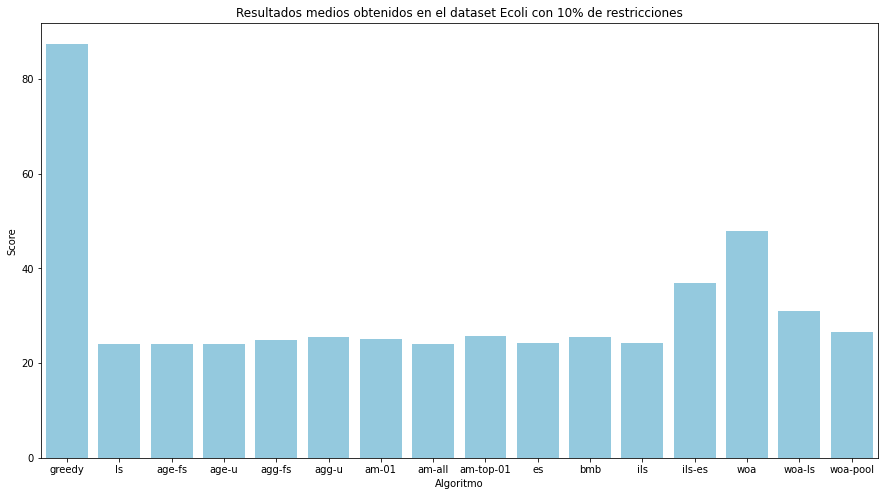
\includegraphics[width=1\textwidth]{images/comparativa}
  \caption{Resultados medios obtenidos para el problema ecoli-10}
\end{figure}

En este cuadro podemos ver de manera visual la diferencia entre los resultados
medios obtenidos para cada algoritmo en el conjunto más complejo, ecoli-10. Como
se puede apreciar ha habido una evolución positiva entre las distintas mejores
que hemos implementado, siendo el uso de la búsqueda local la versión que más a
mejorado los resultados. Como muestran los datos en crudo si hemos encontrado
soluciones muy buenas con esta versión como por ejemplo la que encuentra la
semilla 699 pero la tendencia es a encontrar soluciones en general de peor
calidad que otras técnicas que hemos visto en la asignatura.

\section{Modificación III: Operadores de cruces}

Tras pensar posibles soluciones para mejorar más la metaheurística me decanté
por buscar en la literatura sobre modificaciones de otros autores a la misma.
En concreto encontré \cite{tabu} donde se proponen dos operadores de cruce para mejorar las
características de explotación-diversificación del algoritmo. Me decanté por
implementar esta versión ya que tenía algunas ideas que yo había considerado
como mantener una lista de mejores soluciones y pensé que podría aportar algo
interesante al estudio.

En el algoritmo al final de cada iteración se decide con una probabilidad del
cincuenta por ciento entre una de los dos operadores siguientes

\begin{algorithm}[H]
  \caption{Intensificación por cruce}
  \label{intensificacion}
  \begin{algorithmic}[1]
    \Procedure{intensificación}{}
    \For{$i \in 0\dots\eta$}
    \State Seleccionamos una ballena aleatoria $X_i$
    \State seleccionamos una ballena $X^*$ aleatoria del conjunto de mejores ballenas 
    \For{$j \in 0\dots\alpha$ centroides aleatorios}
    \State Replazar el centroide $C_j$ de $X_i$ por el centroide $-C_j$ de $X^*$
    \EndFor
    \EndFor    
    \EndProcedure
\end{algorithmic}
\end{algorithm}

\begin{algorithm}[H]
  \caption{diversificación por cruce}
  \label{diversificacion}
  \begin{algorithmic}[1]
    \Procedure{Diversificación}{}
    \For{$i \in 0\dots\eta$}
    \State Seleccionamos una ballena aleatoria $X_i$
    \State seleccionamos otra ballena $X_{rand}$ aleatoria del conjunto de ballenas 
    \For{$j \in 0\dots\alpha$ centroides aleatorios}
    \State Remplazar el centroide $C_j$ de $X_i$ por el centroide $-C_j$ de $X_{rand}$
    \EndFor
    \EndFor    
    \EndProcedure
\end{algorithmic}
\end{algorithm}

La versión del algoritmo introduciendo estos cambios sería 

\begin{algorithm}[H]
  \caption{Whale optimization Algorithm + LS + Cruces}
  \label{alg-lsearch}
  \begin{algorithmic}[1]
    \Procedure{WOA-SHAKE}{max\_evaluaciones}
    \State whales: Inicializar un conjunto de ballenas con k centroides aleatorios
    \State Evaluamos las diferentes ballenas usando nuestra métrica 
    \State Seleccionamos $X^*$ la mejor ballena
    \State Guardamos la mejor solución encontrada al problema
    \State evaluaciones $\leftarrow$ 0
    \While {evaluaciones $<$ max\_evaluaciones }
    \State actualizamos el parámetro $a$
    \For{agente en la lista de ballenas}
    \State Determinar $p$ y calcular  $A$ y $C$.
    \If{$p<0.5$}
    \If {$|A| < 1$}
    \State Movemos la ballena usando el movimiento rectilíneo \eqref{eq:1}
    \ElsIf {$|A|>1$} 
    \State Movimiento rectilíneo usando una ballena aleatorio
    \EndIf
    \Else
    \State Movimiento en espiral utilizando \eqref{eq:2}
    \EndIf
    \EndFor 
    \State Comprobar si alguna solución se ha salido de los limites del problema
    \State Incrementar evaluaciones en el número de evaluaciones correspondiente
    
    \State Evaluar las soluciones encontradas y actualizar la mejor ballena 

    \If{no se ha producido mejora en las ultimas $\lambda$ evaluaciones}
    \If{numero aleatorio $<$ 0.5}
    \State Aplicar Intensificación \ref{intensificacion}
    \Else
    \State Aplicar Diversificación \ref{diversificacion}
    \EndIf
    \EndIf    
    \If{la mejor ballena es la mejor solución encontrada}
    \State Actualizar la mejor solución encontrada hasta el momento
    \EndIf

    \EndWhile
    \State
    \Return Construir la solución asociada a la mejor ballena encontrada
    \EndProcedure
  \end{algorithmic}
\end{algorithm}

\subsection{Experimentación}

\begin{figure}[H]
  \begin{subfigure}{.5\textwidth}
    \centering
    % include first image
    \begin{table}[H]
      \centering
      \resizebox{\textwidth}{!}{
        \begin{tabular}{l|l|l|l|l|}
\cline{2-5}
& \multicolumn{1}{c|}{Iris} & \multicolumn{1}{c|}{Ecoli} & \multicolumn{1}{c|}{Rand} & \multicolumn{1}{c|}{Tyroid}  \\ \hline 
\multicolumn{1}{|l|}{Semilla 37 } &  0.702643  & 13.131901   &  0.753491   &  13.674530 \\ \hline
\multicolumn{1}{|l|}{Semilla 42 } &  0.694527  & 13.163324   &  0.753899   &  13.822516 \\ \hline
\multicolumn{1}{|l|}{Semilla 440 } &  0.667115  & 13.557816   &  0.730190   &  14.170967 \\ \hline
\multicolumn{1}{|l|}{Semilla 699 } &  0.691813  & 13.159453   &  0.724393   &  12.865167 \\ \hline
\multicolumn{1}{|l|}{Semilla 752 } &  0.684174  & 13.110302   &  0.745357   &  13.140634 \\ \hline
\multicolumn{1}{|l|}{ Media } &  0.688055  & 13.224559   &  0.741466   &  13.534763 \\ \hline
\end{tabular}
      }                
    \end{table} 
    \caption{Distancia intracluster}
  \end{subfigure}
  \begin{subfigure}{.5\textwidth}
    \centering
    % include second image
    \begin{table}[H]
      \centering
      \resizebox{\textwidth}{!}{
        \begin{tabular}{l|l|l|l|l|}
\cline{2-5}
& \multicolumn{1}{c|}{Iris} & \multicolumn{1}{c|}{Ecoli} & \multicolumn{1}{c|}{Rand} & \multicolumn{1}{c|}{Tyroid}  \\ \hline 
\multicolumn{1}{|l|}{Semilla 37 } &  65.000000  & 1365.000000   &  34.000000   &  343.000000 \\ \hline
\multicolumn{1}{|l|}{Semilla 42 } &  74.000000  & 1346.000000   &  23.000000   &  307.000000 \\ \hline
\multicolumn{1}{|l|}{Semilla 440 } &  77.000000  & 1361.000000   &  35.000000   &  324.000000 \\ \hline
\multicolumn{1}{|l|}{Semilla 699 } &  58.000000  & 1334.000000   &  27.000000   &  349.000000 \\ \hline
\multicolumn{1}{|l|}{Semilla 752 } &  77.000000  & 1364.000000   &  28.000000   &  415.000000 \\ \hline
\multicolumn{1}{|l|}{ Media } &  70.200000  & 1354.000000   &  29.400000   &  347.600000 \\ \hline
\end{tabular}
      }                
    \end{table}  
    \caption{Infeasibility}
  \end{subfigure}

  \begin{subfigure}{.5\textwidth}
    \centering
    \begin{table}[H]
      \centering
      \resizebox{\textwidth}{!}{
        \begin{tabular}{l|l|l|l|l|}
\cline{2-5}
& \multicolumn{1}{c|}{Iris} & \multicolumn{1}{c|}{Ecoli} & \multicolumn{1}{c|}{Rand} & \multicolumn{1}{c|}{Tyroid}  \\ \hline 
\multicolumn{1}{|l|}{Semilla 37 } &  1.114942  & 49.754234   &  0.998346   &  26.218475 \\ \hline
\multicolumn{1}{|l|}{Semilla 42 } &  1.163914  & 49.275894   &  0.919536   &  25.049892 \\ \hline
\multicolumn{1}{|l|}{Semilla 440 } &  1.155531  & 50.072826   &  0.982247   &  26.020058 \\ \hline
\multicolumn{1}{|l|}{Semilla 699 } &  1.059711  & 48.950070   &  0.918836   &  25.628540 \\ \hline
\multicolumn{1}{|l|}{Semilla 752 } &  1.172589  & 49.705803   &  0.947003   &  28.317707 \\ \hline
\multicolumn{1}{|l|}{ Media } &  1.133337  & 49.551765   &  0.953193   &  26.246934 \\ \hline
\end{tabular}
      }                
    \end{table} 
    \caption{Función objetivo}
  \end{subfigure}
  \begin{subfigure}{.5\textwidth}
    \centering
    \begin{table}[H]
      \centering
      \resizebox{\textwidth}{!}{
        \begin{tabular}{l|l|l|l|l|}
\cline{2-5}
& \multicolumn{1}{c|}{Iris} & \multicolumn{1}{c|}{Ecoli} & \multicolumn{1}{c|}{Rand} & \multicolumn{1}{c|}{Tyroid}  \\ \hline 
\multicolumn{1}{|l|}{Semilla 37 } &  29.325428  & 304.140080   &  29.168410   &  55.371357 \\ \hline
\multicolumn{1}{|l|}{Semilla 42 } &  29.487904  & 303.823600   &  29.225350   &  55.270283 \\ \hline
\multicolumn{1}{|l|}{Semilla 440 } &  29.358913  & 303.625240   &  29.203613   &  55.790195 \\ \hline
\multicolumn{1}{|l|}{Semilla 699 } &  29.360378  & 306.017030   &  29.815077   &  56.276577 \\ \hline
\multicolumn{1}{|l|}{Semilla 752 } &  29.720865  & 308.547450   &  29.524380   &  56.064520 \\ \hline
\multicolumn{1}{|l|}{ Media } &  29.450698  & 305.230680   &  29.387366   &  55.754586 \\ \hline
\end{tabular}
      }                
    \end{table} 
    \caption{Tiempo de ejecución}
  \end{subfigure}
  \caption{ Resultados para woa-shake con 10\% de restricciones }
  \label{fig:fig}
\end{figure}
\begin{figure}[H]
  \begin{subfigure}{.5\textwidth}
    \centering
    % include first image
    \begin{table}[H]
      \centering
      \resizebox{\textwidth}{!}{
        \begin{tabular}{l|l|l|l|l|}
\cline{2-5}
& \multicolumn{1}{c|}{Iris} & \multicolumn{1}{c|}{Ecoli} & \multicolumn{1}{c|}{Rand} & \multicolumn{1}{c|}{Tyroid}  \\ \hline 
\multicolumn{1}{|l|}{Semilla 37 } &  0.660507  & 13.302370   &  0.753491   &  13.367699 \\ \hline
\multicolumn{1}{|l|}{Semilla 42 } &  0.661468  & 13.161186   &  0.770779   &  13.754254 \\ \hline
\multicolumn{1}{|l|}{Semilla 440 } &  0.667115  & 13.557816   &  0.738453   &  12.729817 \\ \hline
\multicolumn{1}{|l|}{Semilla 699 } &  0.682628  & 13.386394   &  0.736281   &  12.865167 \\ \hline
\multicolumn{1}{|l|}{Semilla 752 } &  0.684174  & 13.110512   &  0.712756   &  12.891692 \\ \hline
\multicolumn{1}{|l|}{ Media } &  0.671178  & 13.303656   &  0.742352   &  13.121726 \\ \hline
\end{tabular}
      }                
    \end{table} 
    \caption{Distancia intracluster}
  \end{subfigure}
  \begin{subfigure}{.5\textwidth}
    \centering
    % include second image
    \begin{table}[H]
      \centering
      \resizebox{\textwidth}{!}{
        \begin{tabular}{l|l|l|l|l|}
\cline{2-5}
& \multicolumn{1}{c|}{Iris} & \multicolumn{1}{c|}{Ecoli} & \multicolumn{1}{c|}{Rand} & \multicolumn{1}{c|}{Tyroid}  \\ \hline 
\multicolumn{1}{|l|}{Semilla 37 } &  168.000000  & 2769.000000   &  75.000000   &  552.000000 \\ \hline
\multicolumn{1}{|l|}{Semilla 42 } &  143.000000  & 2836.000000   &  29.000000   &  621.000000 \\ \hline
\multicolumn{1}{|l|}{Semilla 440 } &  126.000000  & 2769.000000   &  73.000000   &  707.000000 \\ \hline
\multicolumn{1}{|l|}{Semilla 699 } &  133.000000  & 2830.000000   &  47.000000   &  682.000000 \\ \hline
\multicolumn{1}{|l|}{Semilla 752 } &  153.000000  & 2708.000000   &  38.000000   &  790.000000 \\ \hline
\multicolumn{1}{|l|}{ Media } &  144.600000  & 2782.400000   &  52.400000   &  670.400000 \\ \hline
\end{tabular}
      }                
    \end{table}  
    \caption{Infeasibility}
  \end{subfigure}

  \begin{subfigure}{.5\textwidth}
    \centering
    \begin{table}[H]
      \centering
      \resizebox{\textwidth}{!}{
        \begin{tabular}{l|l|l|l|l|}
\cline{2-5}
& \multicolumn{1}{c|}{Iris} & \multicolumn{1}{c|}{Ecoli} & \multicolumn{1}{c|}{Rand} & \multicolumn{1}{c|}{Tyroid}  \\ \hline 
\multicolumn{1}{|l|}{Semilla 37 } &  1.193085  & 50.447876   &  1.023431   &  23.459171 \\ \hline
\multicolumn{1}{|l|}{Semilla 42 } &  1.114793  & 51.205482   &  0.875156   &  25.107164 \\ \hline
\multicolumn{1}{|l|}{Semilla 440 } &  1.066549  & 50.703323   &  1.001194   &  25.654950 \\ \hline
\multicolumn{1}{|l|}{Semilla 699 } &  1.104252  & 51.350200   &  0.905444   &  25.333258 \\ \hline
\multicolumn{1}{|l|}{Semilla 752 } &  1.169201  & 49.437720   &  0.849526   &  27.334202 \\ \hline
\multicolumn{1}{|l|}{ Media } &  1.129576  & 50.628920   &  0.930950   &  25.377749 \\ \hline
\end{tabular}
      }                
    \end{table} 
    \caption{Función objetivo}
  \end{subfigure}
  \begin{subfigure}{.5\textwidth}
    \centering
    \begin{table}[H]
      \centering
      \resizebox{\textwidth}{!}{
        \begin{tabular}{l|l|l|l|l|}
\cline{2-5}
& \multicolumn{1}{c|}{Iris} & \multicolumn{1}{c|}{Ecoli} & \multicolumn{1}{c|}{Rand} & \multicolumn{1}{c|}{Tyroid}  \\ \hline 
\multicolumn{1}{|l|}{Semilla 37 } &  34.639317  & 355.852940   &  34.618073   &  65.185326 \\ \hline
\multicolumn{1}{|l|}{Semilla 42 } &  34.879158  & 356.064600   &  34.605022   &  65.144990 \\ \hline
\multicolumn{1}{|l|}{Semilla 440 } &  34.592080  & 357.348900   &  34.459778   &  65.300385 \\ \hline
\multicolumn{1}{|l|}{Semilla 699 } &  34.590010  & 360.112240   &  35.237167   &  65.788895 \\ \hline
\multicolumn{1}{|l|}{Semilla 752 } &  34.918400  & 357.927300   &  34.806717   &  66.101330 \\ \hline
\multicolumn{1}{|l|}{ Media } &  34.723793  & 357.461196   &  34.745351   &  65.504185 \\ \hline
\end{tabular}
      }                
    \end{table} 
    \caption{Tiempo de ejecución}
  \end{subfigure}
  \caption{ Resultados para woa-shake con 20\% de restricciones }
  \label{fig:fig}
\end{figure}

\subsection{Resultados}

En general como muestran las tablas anteriores los resultados que proporcionan
esta nueva implementación no mejoran los resultados con los que partíamos del
algoritmo base. El comportamiento que muestran los algoritmos de la modificación
III y el algoritmo base son muy similares y todo apunta a que hay un problema en
el equilibrio entre exploración y explotación, en este caso, por una falta de
explotación de las soluciones. 

No obstante la idea que se presentaba en este artículo era interesante por lo que
como trabajo futuro podría ser interesante sustituir el operador de
intensificación por otro tipo de algoritmo que produzca mejores resultados. 

También podría ser interesante para trabajo futuro modificar el modo en el que
se explora el espacio de soluciones ya que este artículo propone una especia de
simetría de los centroides respecto a los ejes cartesianos y es muy probable que 
esta sea la razón de que no funcione como se espera.

\section{Conclusiones}

En el desarrollo de esta práctica hemos introducido una metaheurística de tipo
PSO para solucionar el problema de clustering con restricciones. Tras solventar
el problema de adaptar la metaheurística al problema hemos visto que las
soluciones no eran buenas pese a que las ideas que se introducen en el algoritmo
resultaban interesantes teóricamente. 

Con las modificaciones introducidas tomadas de ideas que hemos visto a lo largo
del cuatrimestre han permitido que lleguemos a una implementación que mejora las
características de explotación-exploración de la metaheurística para el problema
y que han permitido encontrar resultados óptimos en 3/4 de los problemas y
resultados que podemos considerar bastante buenos para el dataset
\textit{ecoli}.

La implementación de los operadores de cruce, pese a que parecía una idea
alternativa buena para solventar las carencias que hemos analizado en la
metaheurística para este problema, han demostrado no ser tan eficaces.

Se ha demostrado en esta práctica como es importante encontrar un equilibrio
entre explotación y exploración ya que tiene un impacto directo en el
comportamiento de las metaheurísticas y cómo distintas técnicas son más eficaces
que otras en determinados problemas.

\begin{thebibliography}{9}

  \bibitem{woa}
  Seyedali Mirjalili
  \textit{The Whale Optimization Algorithm}
  \url{https://doi.org/10.1016/j.advengsoft.2016.01.008}

  \bibitem{taxonomi}
  \textit{Comprehensive Taxonomies of Nature- and Bio-inspired Optimization: Inspiration versus Algorithmic Behavior, Critical Analysis and Recommendations}
  \url{https://arxiv.org/abs/2002.08136}


  \bibitem{tabu} 
  Kareem Kamal A. Ghany, Amr Mohamed AbdelAziz, Taysir Hassan A. Soliman, Adel Abu El-Magd Sewisy 
  \textit{A hybrid modified step Whale Optimization Algorithm with Tabu Search for data clustering}. 
  \url{https://doi.org/10.1016/j.jksuci.2020.01.015}
  
  \bibitem{matlab}
  Whale Optimization Algorithm Implementation in MATLAB
  \url{https://github.com/AdrikaMukherjee/Whale-Optimization-Algorithm/blob/master/WOA.m}
\end{thebibliography}

\end{document}